%%%%%%%%%%%%%%%%%%%%%%%%%%%%%%%%%%%%%%%%%%%%%%%%%%%%%%%%%%%%%%%%%%%%%%%%%%%%%%%
% 0_simulat.tex                                                               %
% by: David A. Clarke                                                         %
%%%%%%%%%%%%%%%%%%%%%%%%%%%%%%%%%%%%%%%%%%%%%%%%%%%%%%%%%%%%%%%%%%%%%%%%%%%%%%%


% Normal preamble stuff.
\documentclass[12pt]{book}
\usepackage[title]{appendix}
\usepackage{mathtools,tensor,physics,slashed,textcomp,mhchem}
\usepackage{microtype} % should help with hyphenation
\usepackage{bbm} % 4-vectors

% This section is for making C++ code.
\usepackage[dvipsnames]{xcolor}
\usepackage{listings}
\lstset{
  backgroundcolor=\color{gray!10},
  basicstyle=\ttfamily,
  breakatwhitespace=false,
  breaklines=true,
  captionpos=b,
  columns=fullflexible,
  commentstyle=\color{OliveGreen},
  extendedchars=true,
  frame=single,
  keepspaces=true,
  keywordstyle=\color{blue},
  language=c++,
  numbers=none,
  numbersep=5pt,
  numberstyle=\time\color{blue},
  rulecolor=\color{Gray},
  showspaces=false,
  showstringspaces=false,
  showtabs=false,
  stepnumber=5,
  stringstyle=\color{Orchid},
  tabsize=4,
  title=\lstname
}


% davitex and required packages
\usepackage{amsmath,amssymb,graphicx,multirow,tabularx}
\usepackage{davitex}

\newcommand{\fvec}[1]{\mathbbm{#1}}
\newcommand{\units}[1]{\,[\text{#1}]}


% If you click on citations or equation references, you will be take
% to the corresponding page. 
\usepackage{hyperref}
\hypersetup{
  colorlinks=true,
  linkcolor=black,
  citecolor=magenta,
  urlcolor=blue,
}


% Put references at the end of each chapter, directly after the
% end of the chapter, call them "References" instead of
% "Bibliography", and use numbers with square brackets.
\usepackage{url,natbib,chapterbib}
\let\oldbibliography\bibliography
\renewcommand{\bibliography}[1]{{%
  \let\chapter\section%
  \oldbibliography{#1}}}
\renewcommand\bibname{References}
\setcitestyle{numbers,square}


% Make index and let it appear in table of contents.
\usepackage{makeidx}
\makeindex
\usepackage[totoc]{idxlayout}


% Prevent hyphenation.
\setlength\parindent{15pt}
\overfullrule=2cm


% Theorems and stuff.
\usepackage{amsthm}
\usepackage[many]{tcolorbox}
\tcbuselibrary{theorems}
\newtcbtheorem[number within=section]{theorem}{Theorem}{%
  breakable,
  enhanced,
  before skip=10pt,
  colback=green!5,
  colframe=green!35!black,
  fonttitle=\bfseries}{thm}
\newtcbtheorem[number within=section]{proposition}{Proposition}{%
  breakable,
  enhanced,
  before skip=10pt,
  colback=green!5,
  colframe=green!35!black,
  fonttitle=\bfseries}{prp}
\newtcbtheorem[number within=section]{lemma}{Lemma}{%
  breakable,
  enhanced,
  before skip=10pt,
  colback=green!5,
  colframe=green!35!black,
  fonttitle=\bfseries}{lem}
\newtcbtheorem[number within=section]{corollary}{Corollary}{%
  breakable,
  enhanced,
  before skip=10pt,
  colback=green!5,
  colframe=green!35!black,
  fonttitle=\bfseries}{cor}
\newtcbtheorem[number within=section]{example}{Example}{%
  breakable,
  enhanced,
  before skip=10pt,
  colback=blue!5,
  colframe=blue!35!black,
  fonttitle=\bfseries}{cor}
\theoremstyle{definition}
\newtheorem*{defn}{Definition}


% Some environments for some front matter.
\newenvironment{frontstuff}
  {\centering\chapter*{}}
  {\clearpage}
\newenvironment{listofabbrev}
  {\chapter*{List of Abbreviations}}
  {\clearpage}


% Feynman rule references
\definecolor{light}{gray}{.85}
\newcommand{\F}[1]{\colorbox{light}{{F}{#1}}}


% Note that book class by default is formatted to be printed back-to-back.
\title{\bf Simulating Reality: A First Encounter with
Lattice Field Theory for First-Year Undergraduates} 
\author{David Clarke}


\begin{document}
\frontmatter                            % roman page no., suppress chapter
\maketitle                              % print title page


\begin{frontstuff} % ----------------------------------------------- FRONT STUFF

\section*{Symbology}
\begin{tabular}{ll}
$\exists$       & There exists \\
$\forall$       & For all \\
$\in$           & Is a member of the set \\
$\leq$          & Less than or equal to; is a subgroup of\\
$\approx$       & Approximate equality \\
$\equiv$        & Is defined as \\
$\propto$       & Is proportional to \\

$a$             & Lattice spacing \\
$\C$            & Complex numbers \\
$c$             & Speed of light\\
$G$             & Newton's gravitational constant\\
$\hbar$         & Planck's constant \\
$k_B$           & Boltzmann's constant \\
$\log$          & Natural logarithm \\
$\N$            & Natural numbers \\
$N_c$           & Number of colors \\
$N_s$           & Lattice extension in a spatial direction \\
$N_\tau$        & Lattice extension in temperature/Euclidean time direction\\
$\pr{X}$        & Probability of event $X$ \\
$\Q$            & Rational numbers \\
$q$             & Gaussian or Student difference test \\
$\R$            & Real numbers \\
$\SU(N)$        & Special unitary group of degree $N$ \\
$\sigma$        & String tension\\
$\sigma_i$      & A Pauli matrix\\
$T_c$           & Deconfining phase transition temperature\\
$\mathbb{Z}$    & Integers \\


\end{tabular}
\clearpage



\section*{Abbreviations}
\begin{tabular}{ll}
BC      &       Boundary condition \\
CCW     &       Counterclockwise\\
CDF     &       Cumulative distribution function \\
CLT     &       Central limit theorem\\
CW      &       Clockwise\\
EM      &       Electromagnetic\\
FLOP    &       Floating point operation\\
LFT     &       Lattice field theory\\
LGT     &       Lattice gauge theory\\
LQCD    &       Lattice QCD\\
LHS     &       Left hand side\\
LLN     &       Law of large numbers\\
MCMC    &       Markov chain Monte Carlo\\
OOP     &       Object-oriented programming \\
PDF     &       Probability distribution function \\
QCD     &       Quantum chromodynamics \\
QM      &       Quantum mechanics \\
RHS     &       Right hand side \\
RNG     &       Random number generator \\
SM      &       Standard Model \\
s.t.    &       Such that \\
UV      &       Ultraviolet \\
WLOG    &       Without loss of generality
\end{tabular}
\clearpage



\end{frontstuff} % ----------------------------------------------------- PREFACE


\chapter{Acknowledgements}
These notes were developed in part with helpful feedback from students
and friends who had a look at what I wrote.
In particular I would like to thank Grant Curell and my students Kai Ebira
and Daeton McClure for suggestions to help improve the readability of
the notes and make the conveyed information more complete.
Grant especially devoted much time to helping make the discussion about
matrices and multivariable calculus in Chapter 1 more pedagogical.


\chapter{Preface}

Particle physics is the subdiscipline of physics that studies the smallest
particles in existence. Some of these particles are the building blocks of all known
matter, and others are physical manifestations of forces; indeed from the
modern perspective of particle physics, fundamental forces are mediated by
particles called bosons. This is the most fundamental level of nature we
experimentally understand, so in that sense, particle physics studies
the most basic building blocks of reality.

Lattice field theory (LFT) or lattice gauge theory (LGT) is a framework that
allows us to study particle physics using a computer. There are several
strategies for doing particle physics calculations on the market. In some cases
LFT serves as a cross-check of these other approaches. Sometimes, LFT can be
used to compute physical quantities that can't be computed using other methods.

Lattice calculations generate random snapshots of space-time, then measure a
physical quantity, such as a particle mass, on those snapshots. We then
perform statistical analyses on these measurements. Generating the snapshots is 
highly computationally demanding, utilizing in some cases a significant 
fraction of the resources of the most powerful supercomputers in the world. 
Therefore a significant portion of LFT work is focused on high-performance
computing.

The intention of these notes is to give an introduction to LFT that is
readable by a first-year undergraduate in physics. To get a full understanding
of LFT will not be possible for a scientist at this stage in their career, since
LFT lies at the intersection of many fields of math, physics, and computer
science, many of which one will not see until graduate school. Still, my hope is
that the reader can get a heuristic understanding of the field, at least enough
to be able to write scripts that carry out rudimentary statistical analyses on
some physical quantities while having some intuition of what it means.

I attempted to make this text relatively self-contained. However there will be
many parts that I do not explain in detail and must be taken for granted.
Moreover I assume the reader already has had a course with 
\begin{itemize}
  \item calculus (limits, derivatives, and integrals)
  \item energy and momentum conservation
  \item forces
\end{itemize}
Moreover, it is helpful if the reader already knows just a little bit about programming.
This text is developed in tandem with a course that gives first-year
undergraduates some experience in particle physics research, and in that course,
Python is the language of choice.

The layout is pretty simple: There are some preliminary chapters with
hopefully enough additional math and physics to give you a foothold in the lattice
framework. I would recommend not to skip anything in these chapters, even if it
includes things you already know, just so that you can get used to my notation
and so that you can gain a little context why these topics are of interest.
The next chapter is an introduction to the ideas and history of LFT.

One way to gain some familiarity with lattice QCD is to read through these
notes from start to finish. If you are using these notes in the context
of an undergraduate research experience, you can also use it just as
reference material. That is, you can open up a chapter or go to an index
to try to gain some information about a topic or some jargon that is
unfamiliar to you.

\tableofcontents                        % print table of contents
\mainmatter                             % arabic page no., include chapter


% These are the chapters of the book.
\chapter{Some mathematics}\label{ch:group}


In this chapter I just want to show some ideas and notation in math that I am
not sure you have seen yet. {\it It is not crucially important that you understand
anything in this chapter deeply}, but I think it will help orient
yourself in this research to have some idea of what certain terms and symbols
mean, and how they are connected with each other and physics.

In each section, I tried to provide the minimum amount of knowledge that I think is
needed for later sections of the book. Therefore the sections are in no way
complete, and many facts will be stated without proof. To fully understand the
subject matter of each section likely requires you to take a class. Hopefully
these notes will at least help motivate those subjects. You will see some facts
that are important to learn, and their context in physics and other areas of
math.


\section{Preliminary ideas}

We want to discuss math in a fairly abstract way, in part because one of our
goals will be to look at generic mathematical structures. At the end of the book 
we will look at groups, structures that have only three characteristics. We will
 see that many math structures you've already encountered are examples of 
groups\footnote{In
general this is quite powerful, because if you know a fact about a group, and
you know further that a math structure is a group, you immediately know that
fact about that structure. We will not really leverage this power in this book;
I just want you to get acquainted with notation and ideas.}.
Hence we will need some notation that is agnostic to any particular math
structure.

To start, a {\it set}\index{set} is a collection of objects of
any kind, anything\footnote{This is technically wrong. It turns out that one has
to be very careful how a set is defined. Bertrand Russell was the first do
discover this; if you are interested in what can go wrong, look up 
Russell's\index{Russell's paradox}
paradox. For our purposes, this subtlety won't matter.}
you can think of. Everyone in the room you're in forms a set. The counting
numbers form a set. The symmetries of a ball form a set. We usually denote a set
with curly brackets
\begin{equation}
A=\{1,2,3,4\}.
\end{equation}
This means that $A$ is the set containing the numbers 1, 2, 3, and 4.
The things that the set contains are called {\it elements}\index{element}
or\index{member} {\it members}, and we indicate that, e.g. 1 is an element of
$A$ by writing
\begin{equation}
1\in A,
\end{equation}
which we read as ``1 is an element/member of the set $A$" or ``1 is in $A$".
If we want to refer to an arbitrary element $a$ of $A$, we write
\begin{equation}
a\in A,
\end{equation}
and if we want to say that $b$ is not a member of $A$, we write
\begin{equation}
b\notin A,
\end{equation}
The number of elements in a finite set is called its\index{cardinality}
{\it cardinality}. The cardinality of the set $A$ above is 4, and we write
\begin{equation}
  |A|=4.
\end{equation}
A {\it finite} set has a finite cardinality; otherwise it's an infinite set.

It is also useful to introduce an organizational hierarchy for sets. For
instance the set
\begin{equation}
  B=\{1,2,3,4,5,6\}
\end{equation}
is larger than $A$, but it contains $A$ entirely. We write
\begin{equation}
A\subset B.
\end{equation}
Talking about set logic is a good opportunity to introduce some more notation.
It is common to use $\Forall$ as shorthand for ``for all" or ``for any".
Since $A\subset B$, we know that $\Forall a\in A$ we must have $a\in B$.
To express that last idea, we write
\begin{equation}\label{eq:subsetIn}
a\in A\Rightarrow a\in B.
\end{equation}
The\index{set!empty} {\it empty set} $\emptyset$ is the set with nothing in it
at all. If a set has at least one element, it is\index{nonempty} {\it nonempty}.
From \equatref{eq:subsetIn} it follows that for any set $C$
\begin{equation}
\emptyset\subset C~~~~\text{and}~~~~C\subset C.
\end{equation}


\begin{example*}{}{}
  This example serves to introduce some notation for some infinite 
  sets you're likely already familiar with.
  \begin{enumerate}
    \item $\N$ is our symbol for the\index{number!natural} {\it natural
          numbers}, i.e. the infinite set
          $$ \N=\{1,2,3,...\}. $$
    \item $\Z$ represents the\index{integers} {\it integers}, i.e. the infinite
          set
          $$ \Z=\{...,-3,-2,-1,0,1,2,3,...\}. $$
    \item The\index{number!rational} {\it rational numbers} $\Q$ are the 
          infinite set of
          fractions formed using integers, of course not allowing 0 to be in the
          denominator. We write
          $$ \Q=\left\{\frac{m}{n} \suchthat  m,n\in \Z~\text{and}~n\neq0\right\}. $$
          In the above, s.t. is shorthand for the phrase ``such that".
    \item The\index{number!real} {\it real numbers} $\R$ include, in addition to the
          rationals, numbers that cannot be expressed as a fraction of integers.
          These include numbers like $\sqrt{2}$ as well as numbers like
          $e$ and $\pi$. It is a major digression to write $\R$ in set notation,
          whose construction is achieved canonically by starting with the rationals, 
          so we'll just leave it at that.
    \item Define $i\equiv\sqrt{-1}$. The\index{number!complex} {\it complex
          numbers} are an extension of the reals allowing for roots of negative
          numbers. It is given by
          $$ \C=\{x+iy \suchthat x,y\in\R \}. $$
          Given a complex number $z=x+iy$, its {\it complex
          conjugate}\index{complex conjugate} $z^*$ is defined by
          $$ z^*\equiv x-iy.$$
          Since you need two independent real numbers to describe a complex
          number, you can visualize complex numbers as lying in a plane. A
          measure of the ``size" of a complex number is its distance from 
          the origin or its {\it magnitude}. This is given by
          $$ |z| = \sqrt{zz^*} = \sqrt{x^2+y^2}. $$
    \item $\N\subset \Z \subset \Q \subset \R \subset \C$.
          
  \end{enumerate}
\end{example*}


We can introduce the notion of a function. A\index{function} 
{\it function} or\index{map} {\it mapping} $f$ between $X$ and $Y$ 
associates $\Forall x\in X$ a unique element $f(x)\in Y$. We 
write
\begin{equation}
f:X\to Y.
\end{equation}
Usually $X$ is called the\index{domain} {\it domain} 
and $Y$ is called the\index{codomain} {\it codomain}.
The\index{image} {\it image} or\index{range} {\it range}
is $f(X)$, i.e. the set of all values $f$
 maps to given the domain. Note $f(X)\subset Y$.

Next we classify a few different kinds of functions.
A function is\index{injection} {\it injective}
or\index{one-to-one} {\it one-to-one} if each element in $X$
maps to a different element in $Y$. We can express this symbolically as
\begin{equation}
 \Forall x_1,x_2\in X,~f(x_1)=f(x_2)\Rightarrow x_1=x_2.
\end{equation}
A\index{surjection} {\it surjective} or\index{onto} {\it onto} function 
maps to every possible element of the codomain $Y$. Symbolically,
\begin{equation}
 \Forall y\in Y,~\Exists x\in X \suchthat y=f(x), 
\end{equation}
where we have introduced the symbol $\Exists$ as shorthand for ``there is at
least one" or ``there exists". Finally a function is\index{function!bijective}
{\it bijective} if it is both an injection and a surjection. In this case each
element of $X$ corresponds to exactly one element of $Y$, and vice-versa.
Pictorial representations of these kinds of functions are shown in
\figref{fig:mapping}.

\begin{figure}
\centering
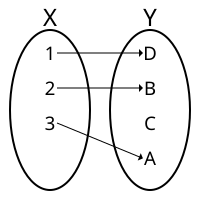
\includegraphics[width=0.45\linewidth]{figs/Injection.png}~~~
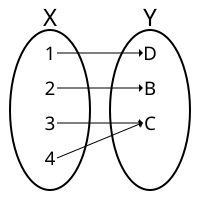
\includegraphics[width=0.45\linewidth]{figs/Surjection.png}\\
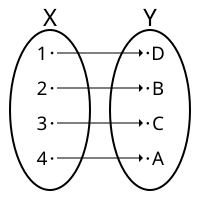
\includegraphics[width=0.45\linewidth]{figs/Bijection.png}~~~
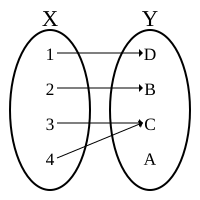
\includegraphics[width=0.45\linewidth]{figs/Not-Injection-Surjection.png}
\caption{Example mappings that are injective (top left), surjective (top right),
bijective (bottom left), and none of these (bottom right). Images taken from 
Wikipedia~\cite{wiki:bijection}.}
\label{fig:mapping}
\end{figure} 

Besides giving the opportunity to show some notation, one useful thing you can
do with bijections is use them to compare set cardinalities. Indeed, if you can
find a bijection $f$ between $X$ and $Y$, you know that $X$ and $Y$ have the
same size. While this is not particularly useful for finite sets, it is useful
for infinite sets, allowing one to classify various kinds of infinity.

\begin{example*}{}{}
Whenever you can find a bijection $f$ between any set $A$ and $\N$, $A$ is said to
be\index{countable} {\it countably infinite}. This infinity, the number
of natural numbers, is usually written\footnote{This symbol is pronounced
``aleph".} as $\aleph_0$, i.e.
$$|\N|=\aleph_0.$$
Intuitively the nomenclature ``countable" makes
sense, since you are using $f$ to assign a single counting number to each
element of $A$. What is perhaps less intuitive is that $\Z$ is countable, i.e.
$$|\Z|=|\N|.$$
So even though $\N$ is fully contained in $\Z$, they have the same size! To see
this, we just need a bijection between $\N$ and $\Z$. Here is one: map every odd
number in $\N$ to the non-negative integers, i.e.
$$ f(1)=0,~f(3)=1,~f(5)=2,~...$$
and so on. Map every even number to the negative integers, i.e.
$$ f(2)=-1,~f(4)=-2,~f(6)=-3,~...$$
etc. This mapping associates exactly one integer to one natural number and vice
versa. It works because it exploits the fact that both sets are infinite. One
can show $\Q$ is also countably infinite, although the mapping is a bit more
subtle\footnote{One can do it for the positive rationals 
by setting up a table where rows represent
numerators and columns denominators. The counting then traces a squiggly path
through the table.}. On the other hand,
$$|\R|>|\N|.$$
This was first shown by Cantor using his so-called ``diagonal argument", which
you can look up if you are interested. The cardinality of the reals is usually
written as $\frak{c}$ and is sometimes called\index{power of the continuum}
the {\it power of the continuum}. This name is extremely badass. It is also
interesting to see that there are, in this sense, different sizes of infinities.
You may sometimes hear people talk about the\index{continuum hypothesis} 
{\it continuum hypothesis}. This hypothesis posits that
there is no set whose cardinality lies between $\aleph_0$ and $\frak{c}$.
Finally we note that any infinity that is not $\aleph_0$ is called {\it
uncountable}\index{uncountable}. Hence we say $\R$ is uncountably infinite.
\end{example*}

\begin{figure}
  \centering
  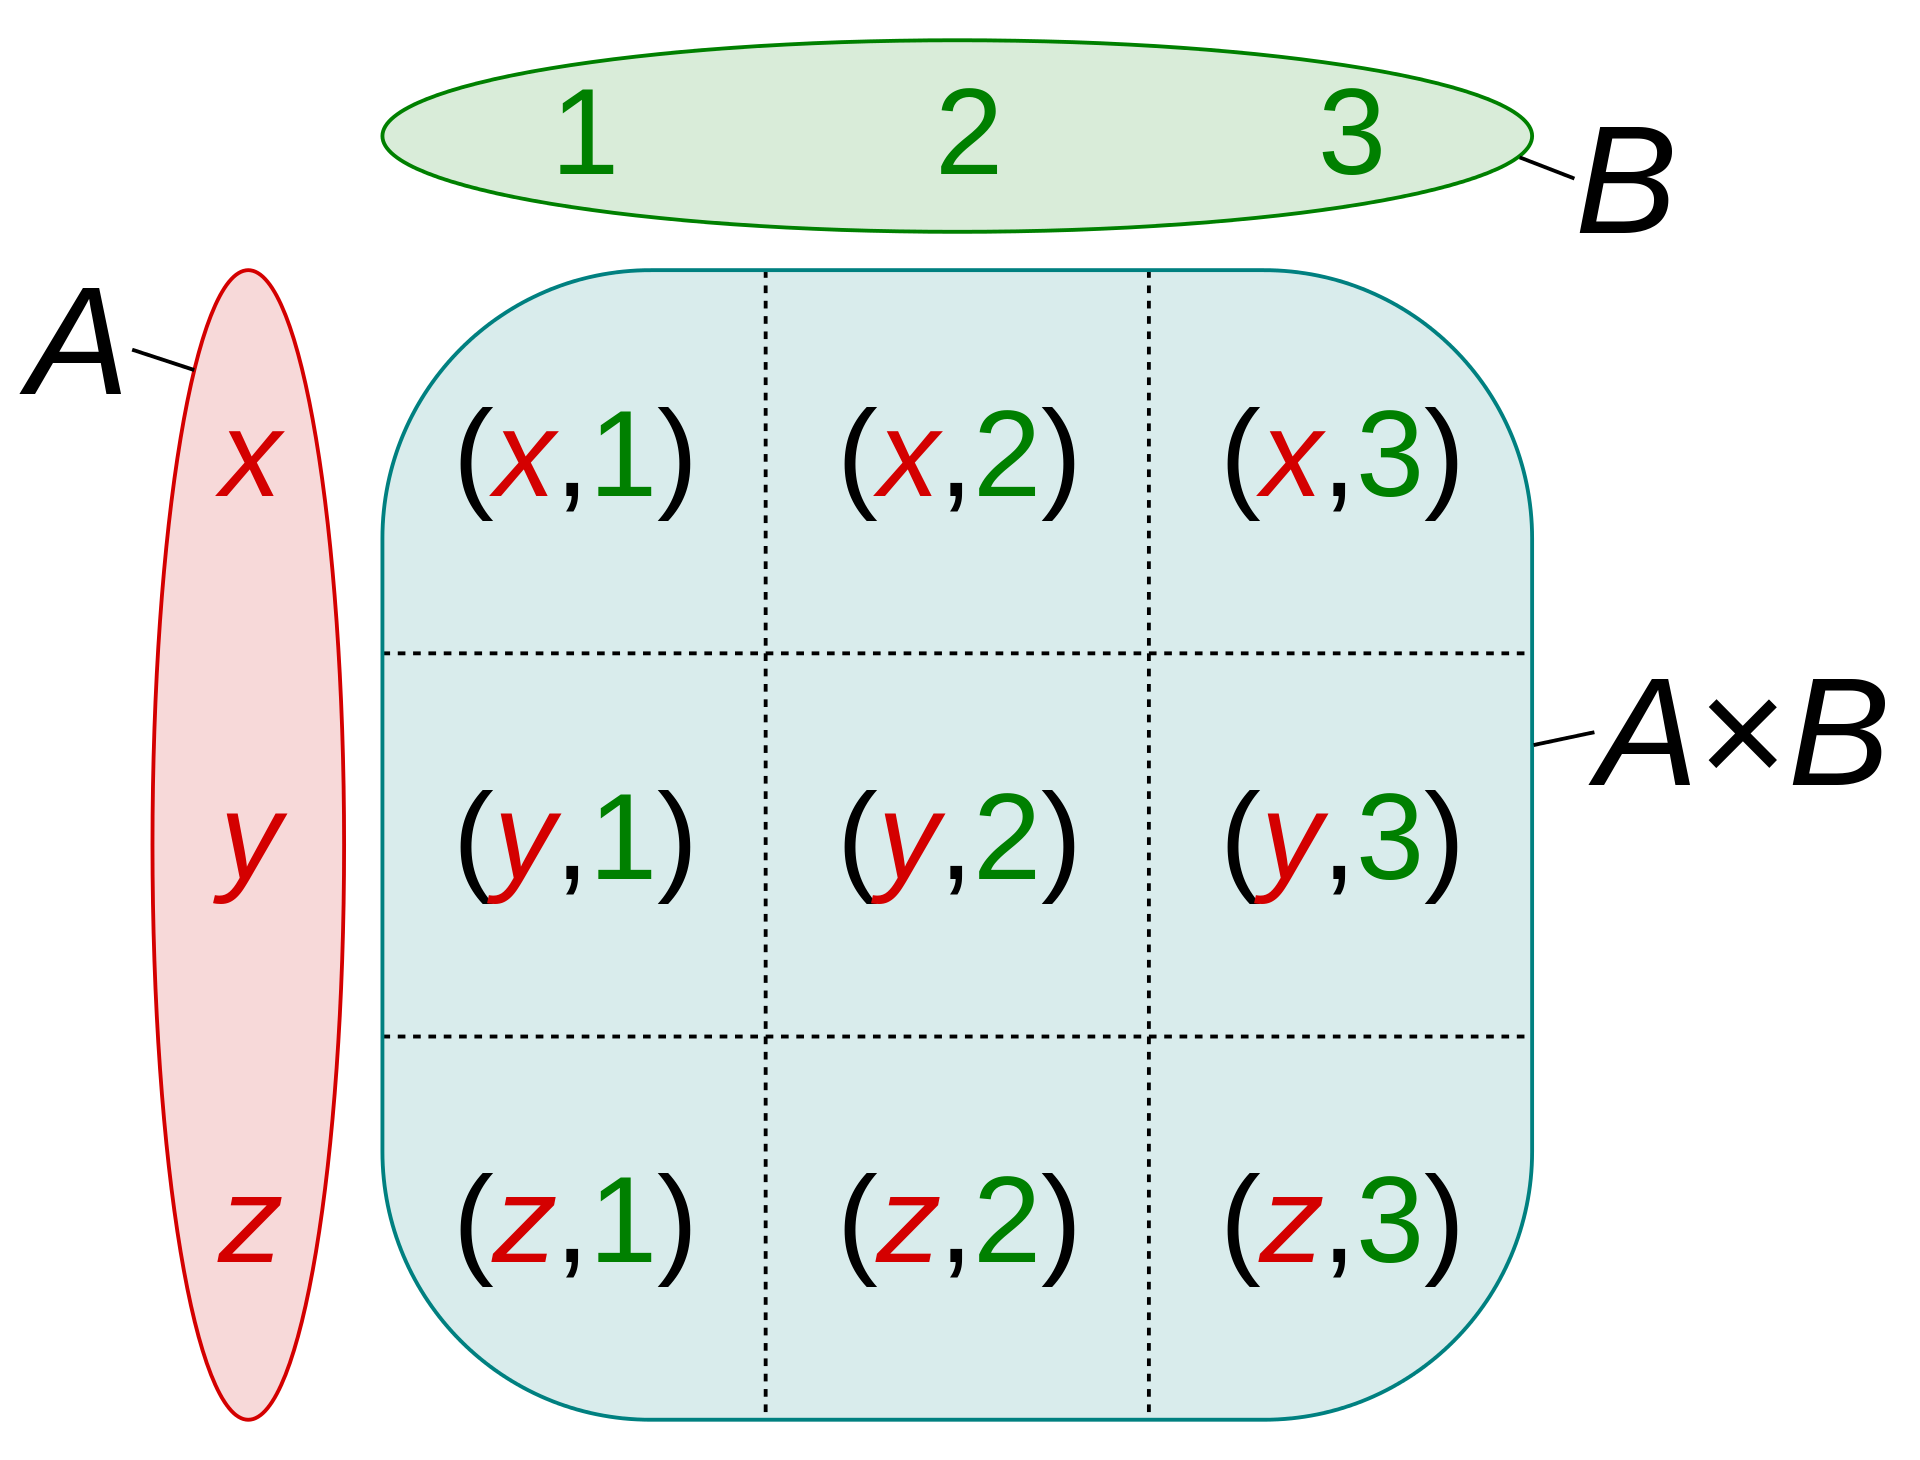
\includegraphics[width=0.45\linewidth]{figs/Cartesian_Product.png}~~~
  \caption{Example of a Cartesian Product. Image taken from 
  Wikipedia~\cite{wiki:cartesian_product}.}
  \label{fig:cartesian_product}
\end{figure} 

To close out the section, we discuss a couple ways of putting sets together.
The most straightforward way is just to ``add" the sets, i.e. form a new set
whose elements include all the elements from the parent sets. For instance if
you have two sets $A$ and $B$, then the\index{union} {\it union} is
\begin{equation}
A\cup B = \{x\suchthat x\in A~\text{or}~x\in B\}.
\end{equation}
You can also create that contains only the elements that both $A$ and $B$ have
in common. This set is the\index{intersection} {\it intersection}
\begin{equation}
A\cap B = \{x\suchthat x\in A~\text{and}~x\in B\}.
\end{equation}
We exist in nature in a space of more than one dimension; therefore it is useful to be
able to combine sets into coordinates. We define the\index{Cartesian product}
{\it Cartesian product} of $A$ and $B$ as the set of tuples
\begin{equation}
A\times B=\{(a,b)\suchthat a\in A~\text{and}~b\in B\}.
\end{equation}
See \figref{fig:cartesian_product} for a visual representation of the Cartesian
product. Later, we will use the Cartesian product to define multi-dimensional spaces.
For instance, a 4-$d$ space can be defined using the set 
\begin{equation}\label{eq:spacetimeSet}
\R^4\equiv\R\times\R\times\R\times\R=\{(x_0,x_1,x_2,x_3)\suchthat
x_0,x_1,x_2,x_3\in\R\}.
\end{equation}


\section{Vectors and matrices}\label{sec:vecmat}

In the last section we looked at many math objects that can be represented by a
single number. If $x\in\Q,\R$, or $\C$, we call\footnote{For this definition of scalar,
we won't let $x\in\N$ or $x\in\Z$ because in nature, we need the number 0 and want to
be able to divide sensibly.} $x$ a\index{scalar} {\it scalar}. 
Thinking ahead to physics, we can express many measurable quantities in nature
as scalars, for instance the temperature.

Some quantities also need to be represented with a direction, quantities such as
the gravitational force. To accomplish that we introduce a tuple of length $n\in\N$,
\begin{equation}\label{eq:vecDef}
  v=\colvec{4}{v_1}{v_2}{\vdots}{v_n},
\end{equation}
where the $v_i$, $1\leq i\leq n$, are scalars all belonging to the same set $A$, i.e.
\begin{equation}
  v\in \underbrace{A\times A\times ... \times A}_{n\text{ times}} \equiv A^n.
\end{equation}
% DC: This is not a vector since A and B are not the same set, it is
% rather just a "tuple". I am just going to introduce what a vector field is and
% define vectors so this distinction becomes clearer. Sorry for the confusion.
%Again using \figref{fig:cartesian_product} as an example, $n$ would be 2 and
%selecting any two points on the square would create the vector $v$. 
We call $v_i$ the $i\nth$ {\it component}.
We want to be able to add these kinds of quantities and multiply them with
scalars $\alpha\in A$. For example if two people are pushing on a cart with
different forces, we want to be able to mathematically represent their combined
effect. To achieve this, we define addition
component-wise by
\begin{equation}\label{eq:vecAdd}
v+w=
  \colvec{4}{v_1}{v_2}{\vdots}{v_n}+
  \colvec{4}{w_1}{w_2}{\vdots}{w_n}
\equiv
  \colvec{4}{v_1+w_1}{v_2+w_2}{\vdots}{v_n+w_n}.
\end{equation}
{\it Scalar multiplication}\index{multiplication!scalar} is defined by
\begin{equation}\label{eq:vecMult}
\alpha v = \alpha \colvec{4}{v_1}{v_2}{\vdots}{v_n}
    \equiv\colvec{4}{\alpha v_1}{\alpha v_2}{\vdots}{\alpha v_n}.
\end{equation}
Using the properties of the set $A$, one can show 
that these operations are {\it distributive}\index{distributive}, 
i.e. that
\begin{equation}\label{eq:vec_distributive}
(a+b)v = av+bv~~~~\text{and}~~~~a(v+w)=av+aw;
\end{equation}
{\it associative}\index{associative}, i.e. that
\begin{equation}
u+(v+w)=(u+v)+w;
\end{equation}
and {\it commutative}\index{commutative}, i.e. that
\begin{equation}\label{eq:vec_commutative}
v+w=w+v.
\end{equation}
If $v\in A^n$ satisfies all of the properties \equatref{eq:vec_distributive} through 
\eqref{eq:vec_commutative}, $v$ is said to be a {\it vector}\index{vector},
and we call\footnote{Usually in math textbooks you'll also see the requirement
of there being an {\it additive identity}\index{identity!additive} 0, or zero
vector, and a {\it multiplicative identity}\index{identity!multiplicative},
or the number 1. Since we restricted $A$ to be a set of scalars, and since we
further restricted scalars to include only $\Q$, $\R$, and $\C$, these
properties are already guaranteed by definitions~\eqref{eq:vecDef} through
\eqref{eq:vecMult}. Therefore I didn't mention them in the main text.}  
$A^n$ a {\it vector space}\index{vector space}. We call $n$
the {\it dimension} of the vector space.
If $n=2$ or 3, it is common in physics to write instead $\vec{v}$.
If $n=4$, we will use the uncommon notation $\fvec{v}$. 
These are just to help remind the reader what kind of object they are looking
at.

\begin{figure}
  \centering
  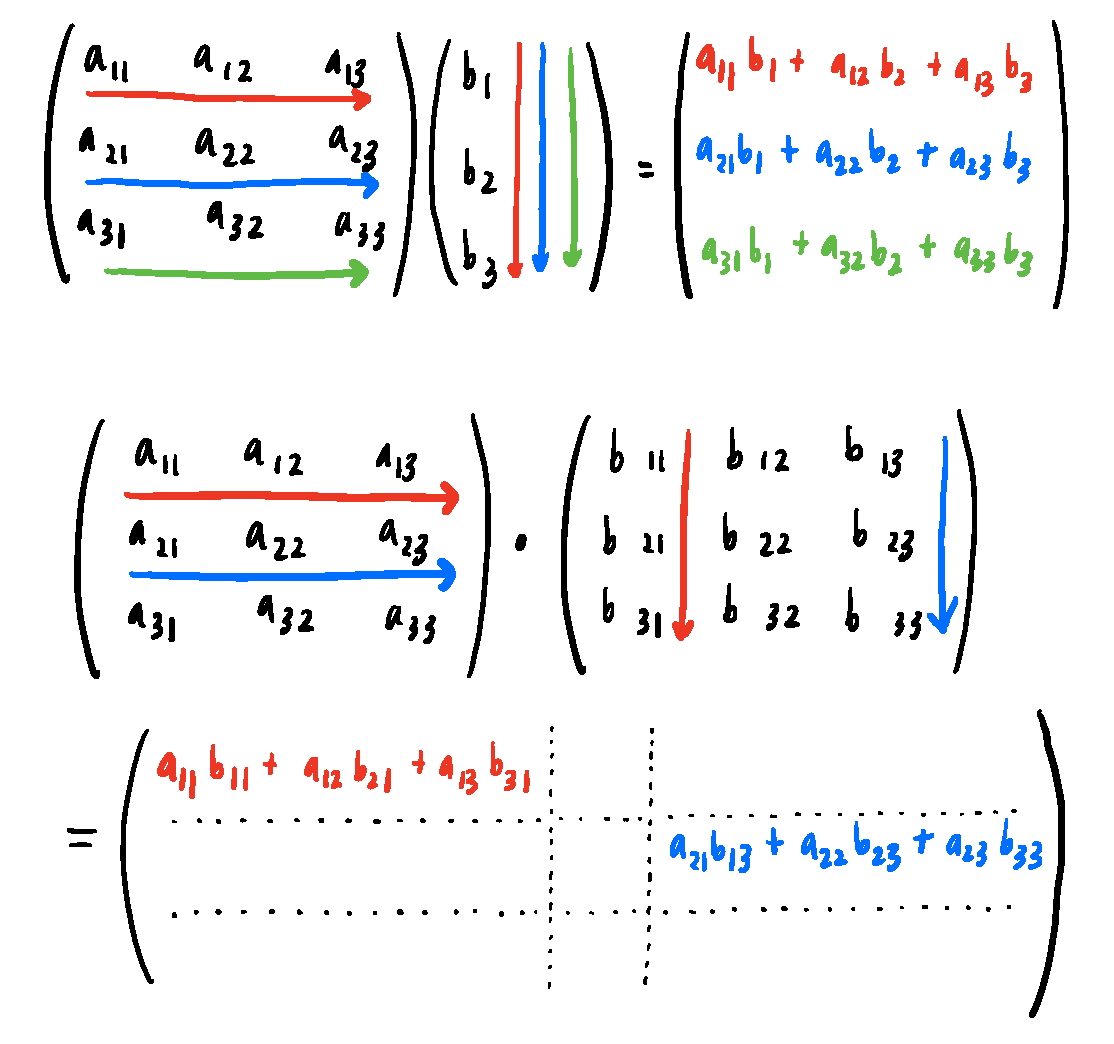
\includegraphics[width=\linewidth]{figs/matrixMult.pdf}
  \caption{Example matrix multiplication for $3\times 3$ matrices. {\it Top}: A
           matrix being applied to a 3D vector. {\it Bottom}: Multiplication of two
           matrices.}
  \label{fig:matrix}
\end{figure}

{\it Matrices} play a fundamental role in physics as well.
We will see they are very useful for understanding different kinds of
symmetries, but they have many other applications as well\footnote{For example
in quantum physics, you will eventually learn that measurable quantities can be
extracted as special, characteristic values of matrices. They can also be used
to solve systems of equations.}. Given a vector space $A^n$, we associate
$n\times n$ matrices\footnote{Such a matrix is usually called a {\it square
matrix}. Matrices don't have to be square matrices, i.e. they can have a
different number of rows than columns. In physics square
matrices matter the most, so that's all we'll worry about for these notes.}, 
which have the form
\begin{equation}\label{eq:basicMatrix}
  M=\left(\begin{array}{cccc}
          a_{11}   & a_{12} &       & a_{1n}\\
          a_{21}   & a_{22} &       & a_{2n}\\
                   &        & \ddots&       \\
          a_{n1}   & a_{n2} &       & a_{nn}
            \end{array}\right). 
\end{equation}
We call each entry $a_{ij}\in A$, $1\leq i,j\leq n$, an {\it element}. The position
of each element is indicated by two subscripts, the left
indicating the row number and the right indicating the column number.
Hence there are $n^2$ elements in a square matrix.

Matrices as defined above\footnote{That is, square matrices. By the way,
in this context of mapping vector spaces into themselves, we sometimes
call matrices {\it operators}\index{operator}.} map $A^n$ into itself, i.e.
\begin{equation}\label{eq:operatorDef}
  M:A^n\to A^n.
\end{equation}
In general, this mapping is achieved through matrix multiplication. If one
multiplies a vector $v$ with a matrix $M$, one gets for the $i\nth$ component
of the product $Mv$
\begin{equation}\label{eq:matTimesVec}
  (Mv)_i=\sum_{j=1}^n a_{ij}v_j,
\end{equation}
where $M$ is our matrix and $v$ is a vector. 

To understand the RHS of \equatref{eq:matTimesVec}, let's look at the example
\begin{equation}\label{eq:matTimesVecEx}
  \left(\begin{array}{cc}
          3   & 4\\ 
          5   & 6\\ 
            \end{array}\right)
  \colvec{2}{1}{-2}
  =\colvec{2}{b_1}{b_2}
\end{equation}
To get the first component of the product,
one starts with the first row of the matrix, multiplying the row's leftmost
element with the vector's first component. Then one adds the next-leftmost
element times the second component, and so on. To get the second component of
the product, one repeats using instead the second row of the matrix.
In our case, we obtain
\begin{equation}\begin{aligned}\label{eq:matMultEx}
  b_1 &= 3\times1 - 4\times2 = -5\\
  b_2 &= 5\times1 - 2\times6 = -7
\end{aligned}\end{equation}
See \figref{fig:matrix} (top) for
a colored representation of what this looks like for a $3\times3$ matrix
multiplying a vector in $\R^3$.

Eqs.~\eqref{eq:operatorDef} and \eqref{eq:matTimesVec} show us that one way to
look at matrices is as functions\footnote{In fact, this perspective is generally 
applicable any time one uses the words ``map" or ``mapping".} that take a vector 
and give back a vector.
For instance \equatref{eq:matMultEx} shows that the matrix in the LHS
of \equatref{eq:matTimesVecEx} maps
\begin{equation}
  \colvec{2}{1}{-2}
  \to\colvec{2}{-5}{-7}.
\end{equation}
Sometimes that perspective is useful, but it is often useful to think about
matrices as math objects in their own right. Matrices can, for instance, be added
together element-wise. 
\begin{equation}\begin{aligned}
  \left(\begin{array}{cccc}
          a_{00}   & a_{01} &       & a_{0n}\\ 
          a_{10}   & a_{11} &       & a_{1n}\\
                   &        &\ddots & \\
          a_{n0}   &        &       & a_{nn} 
  \end{array}\right)
  &+\left(\begin{array}{cccc}
          b_{00}   & b_{01} &       & b_{0n}\\ 
          b_{10}   & b_{11} &       & b_{1n}\\
                   &        &\ddots & \\
          b_{n0}   &        &       & b_{nn} 
  \end{array}\right)\\
  &=\left(\begin{array}{cccc}
          a_{00}+b_{00}   & a_{01}+b_{01} &        & a_{0n}+b_{0n}\\ 
          a_{10}+b_{10}   & a_{11}+b_{11} &        & a_{1n}+b_{1n}\\ 
                          &               & \ddots & \\
          a_{n0}+b_{n0}   &               &        & a_{nn}+b_{nn} 
  \end{array}\right)
\end{aligned}\end{equation}
Analogously as with many kinds of number systems, it is useful to introduce
in $n$ dimensions an additive identity\index{identity!additive} or zero matrix as
\begin{equation}
  \zd_n=\left(\begin{array}{cccc}
          0   & 0 &       & 0\\
          0   & 0 &       & 0\\
              &   & \ddots& \\
          0   &   &       & 0
            \end{array}\right), 
\end{equation}
i.e. it's the $n\times n$ matrix with 0 in every element. With our definition
of matrix addition, we find that for any $n\times n$ matrix $M$
\begin{equation}
\zd_n+M=M+\zd_n=M.
\end{equation}

Besides addition, it is useful to be able to carry out multiplication.
The simplest kind is scalar multiplication\index{multiplication!scalar},
which is defined similarly as with vectors. In particular if $\alpha\in A$,
then
\begin{equation}
  \alpha\left(\begin{array}{cccc}
          a_{00}   & a_{01} &       & a_{0n}\\ 
          a_{10}   & a_{11} &       & a_{1n}\\
                   &        &\ddots & \\
          a_{n0}   &        &       & a_{nn} 
  \end{array}\right)\equiv
  \left(\begin{array}{cccc}
          \alpha a_{00}   & \alpha a_{01} &       & \alpha a_{0n}\\ 
          \alpha a_{10}   & \alpha a_{11} &       & \alpha a_{1n}\\
                          &               &\ddots &  \\
          \alpha a_{n0}   &               &       & \alpha a_{nn} 
  \end{array}\right).
\end{equation}
One can also multiply a matrix $M$ and a matrix $L$. If $L$ has elements
$b_{ij}$, then the product $ML$ is defined element-wise by
\begin{equation}
  (ML)_{ij}=\sum_{k=1}^n a_{ik}b_{kj}.
\end{equation}
Again, this is not particularly easy\footnote{If you still found this explanation confusing, 
this \href{https://youtu.be/kT4Mp9EdVqs}{Khan academy tutorial}
may help.}
to read, so I show this visually for 3 dimensions in
\figref{fig:matrix} (bottom). 
You may be inclined to think that the above 
{\it matrix multiplication}\index{multiplication!matrix} behaves like normal
multiplication, but that is not the case. Most notably, it is not 
in general commutative.
For example
\begin{equation}
  \left(\begin{array}{cc}
          1   & 0\\ 
          0   & 0\\ 
            \end{array}\right)
  \left(\begin{array}{cc}
          0   & 1\\ 
          0   & 0\\ 
            \end{array}\right)
  =\left(\begin{array}{cc}
          0   & 1\\ 
          0   & 0\\ 
            \end{array}\right)
\end{equation}
but
\begin{equation}
  \left(\begin{array}{cc}
          0   & 1\\ 
          0   & 0\\ 
            \end{array}\right)
  \left(\begin{array}{cc}
          1   & 0\\ 
          0   & 0\\ 
            \end{array}\right)
  =\left(\begin{array}{cc}
          0   & 0\\ 
          0   & 0\\ 
            \end{array}\right).
\end{equation}

Again to continue our analogy with other number systems,
we introduce a multiplicative identity for matrices.
In $n$ dimensions, the {\it identity matrix} is
\begin{equation}
  \id_n=\left(\begin{array}{cccc}
          1   & 0 &       & 0\\
          0   & 1 &       & 0\\
          0   &   & \ddots& \\
          0   &   &       & 1
            \end{array}\right), 
\end{equation}
i.e. it is the matrix with 1 along the diagonal and 0 everywhere else. Using
matrix multiplication you can show that for any $n\times n$ matrix $M$
\begin{equation}
  M\id_n =\id_n M = M.
\end{equation}
That is to say, no matter which way you multiply a matrix by $\id_n$, 
you will always get the matrix back. 
%This may seem trivial, but the concept of the
%identity matrix is important and is used extensively in linear algebra. For
%example, it can be used to describe the standard basis which you can then use to
%define linear transformations. You don't need to know what all that is right
%now, but I want to drive home that we are introducing these definitions now to
%build on them later.
Sometimes a matrix is {\it invertible}, i.e. $\Exists M^{-1}$ so that
\begin{equation}
  M^{-1} M=\id_n. 
\end{equation}
We will not discuss strategies for matrix inversion in these short notes, but
finding matrix inverses, and indeed sometimes determining whether a matrix has
an inverse at all, is a topic deserving of a chapter on its 
own\footnote{In fact, some of the most important problems supercomputers work
on revolve around inverting matrices. For example, many machine learning
algorithms require the inversion of large matrices. In the context
of physically realistic lattice calculations, extremely large matrices must be
inverted many, many times to generate space-time snapshots and to measure
certain observables.}. 

Using the above definitions, one can show that for $\alpha,\beta\in A$
and $n\times n$ matrices $O$, $L$ and $M$ that
\begin{equation}\begin{aligned}
(\alpha+\beta)M&=\alpha M+\beta M,\\
\alpha(L+M)&=\alpha L+\alpha M,\\
L+M&=M+L,\\
O+(L+M)&=(O+L)+M.
\end{aligned}\end{equation}
These are most of the usual properties of being distributive, associative,
and having additive commutativity.
Again, importantly, matrix multiplication is in the general case not
commutative.\index{distributive}\index{associative}\index{commutative}

To round out this discussion of thinking about matrices as math objects in their
own right, it is sometimes useful to define functions of matrices.
For starters, we can always
raise a matrix to an arbitrary power $k\in\N$. Hence we have well defined
functions of the form
\begin{equation}
f(M)=M^k\equiv\underbrace{M\,M\,...\,M}_{k\text{ times}},
\end{equation}
and as with ordinary numbers, we define $M^0\equiv \id_n$.
Using scalar multiplication and matrix addition, we are therefore also
able to sensibly define polynomials of matrices
\begin{equation}
f(M)=\alpha_0\id_n + \alpha_1 M + \alpha_2 M^2...+\alpha_n M^n.
\end{equation}
The fact that we can construct polynomials out of matrices empowers us
to define even more general functions through their Taylor series.
For example, the exponential $\exp:\R\to\R$ is given through its Taylor expansion
as
\begin{equation}
\exp(x)=\sum_{i=0}^\infty \frac{x^k}{k!}.
\end{equation}
This allows us to define the exponential of a matrix as
\begin{equation}\label{eq:expMat}
\exp(M)=\sum_{i=0}^\infty \frac{M^k}{k!}.
\end{equation}
All the typical elementary functions $\sin$, $\sinh$, and so on can be
analogously defined on matrices.

Finally, I am obligated to introduce some notation one frequently encounters
in physics with regard to matrices. The {\it trace}\index{trace} of an 
$n\times n$ matrix is the sum of its diagonal elements,
\begin{equation}
  \tr M=\sum_i^nM_{ii}.
\end{equation}
When you {\it transpose}\index{transpose} a matrix, you interchange all of its
off-diagonal elements; i.e. the $i,j$-element gets replaced with the
$j,i$-element, and vice-versa. For example the transpose $M^t$ of the matrix in
\equatref{eq:basicMatrix} is given by
\begin{equation}
  M^t=\left(\begin{array}{cccc}
          a_{11}   & a_{21} &       & a_{n1}\\
          a_{12}   & a_{22} &       & a_{n2}\\
                   &        & \ddots&       \\
          a_{1n}   & a_{2n} &       & a_{nn}
            \end{array}\right). 
\end{equation} 
The {\it complex conjugate}\index{complex conjugate} 
of a matrix simply conjugates all its elements, i.e.
\begin{equation}
  M^*=\left(\begin{array}{cccc}
          a_{11}^*   & a_{12}^* &       & a_{1n}^*\\
          a_{21}^*   & a_{22}^* &       & a_{2n}^*\\
                     &          & \ddots&         \\
          a_{n1}^*   & a_{n2}^* &       & a_{nn}^*
            \end{array}\right). 
\end{equation}
Finally we will sometimes need the conjugate-transpose or 
{\it adjoint}\index{adjoint} of a matrix, which is indicated with a 
little dagger\footnote{Hence we sometimes say ``$M$-dagger".},
$M^\dagger$. It is
\begin{equation}
M^\dagger\equiv (M^*)^t.
\end{equation}
A matrix is said to be {\it unitary}\index{unitary} if
\begin{equation}
M^\dagger M=MM^\dagger=\id_n,
\end{equation}
i.e. unitary matrices are those whose inverses are the same as 
their adjoints.

\section{Calculus with many variables}

In your first encounter with calculus, you likely considered
functions that accept a single real number and then
produce a real number, i.e. functions
\begin{equation}
f:\R\to\R.
\end{equation}
Indeed, this is likely how you have looked at functions for the
majority of your mathematical career. However, a function can also consist of
many real inputs which produce many real outputs. Multivariable calculus is then
the generalization of calculus, where functions can
accept a list of numbers.
Formally\footnote{For example the function $f:\R^2\to\R$
maps a point on the 2-$d$ plane to a point on the number line.}, 
we allow 
\begin{equation}
f:\R^n\to\R,
\end{equation}
where $n\in\N$.
We want to gain some intuition about what it means to take derivatives
of $f$ and to integrate it.

Suppose for a moment we fix $y$, i.e. we don't let $y$ change. This defines a
new function $g$
\begin{equation}\label{eq:fixG}
g(x)\equiv f(x,y)\,\suchthat\text{ $y$ is held constant}.
\end{equation}
Since $g$ is now a function of $x$ only, we can take a derivative\footnote{I'm
being a bit hand-wavy here. It is of course important that your function behaves
nicely in a particular way that you will learn when you take a course in
multivariable calculus. In these notes we will assume the functions we deal with
can be differentiated or integrated unless otherwise stated.} w.r.t. 
$x$ in the familiar way. This defines the {\it partial derivative of $f$ with
respect to $y$}\index{partial derivative}:
\begin{equation}\label{eq:pdv}
\pdv{f(x,y)}{x}\equiv\frac{\dd g(x)}{\dd x}.
\end{equation}
Sometimes as shorthand we write $\partial_x f$ to indicate the above derivative. 
The partial derivative thus effectively treats $y$ as
if it were just another constant. 
Hence partial derivative isolates $x$ to see how $f$
changes when you vary $x$ alone\footnote{It is important for this kind of
thinking that there is no hidden dependence between $x$ and $y$. If $y=h(x)$ one
has to keep track of that, and be a bit careful.}. This is a crucial
manipulation to be able to do in the context of an experiment: One can imagine
having many knobs to turn and wanting to understand to effect of turning each of
them.

Let's try to understand this through a simple example, 
the function $z(x,y)=x^{2}+xy+y^{2}$. It has two inputs, $x$ and $y$. Both $x$ and
$y$ have some impact on the final output $z$. By taking the derivative
$\partial_x z=2x+y$, we learn how $x$
affects $z$ while not allowing $y$ to change.
A plot of $z$ as a function of $x$ and $y$
is shown as the blue surface in \figref{fig:partial_derivative}.
The red line indicates $z$ when we fix $y=1$. At $y=1$,
$\partial_x z(x)$ then corresponds to a tangent line to
the red curve at $x$.

\begin{figure}
  \centering
  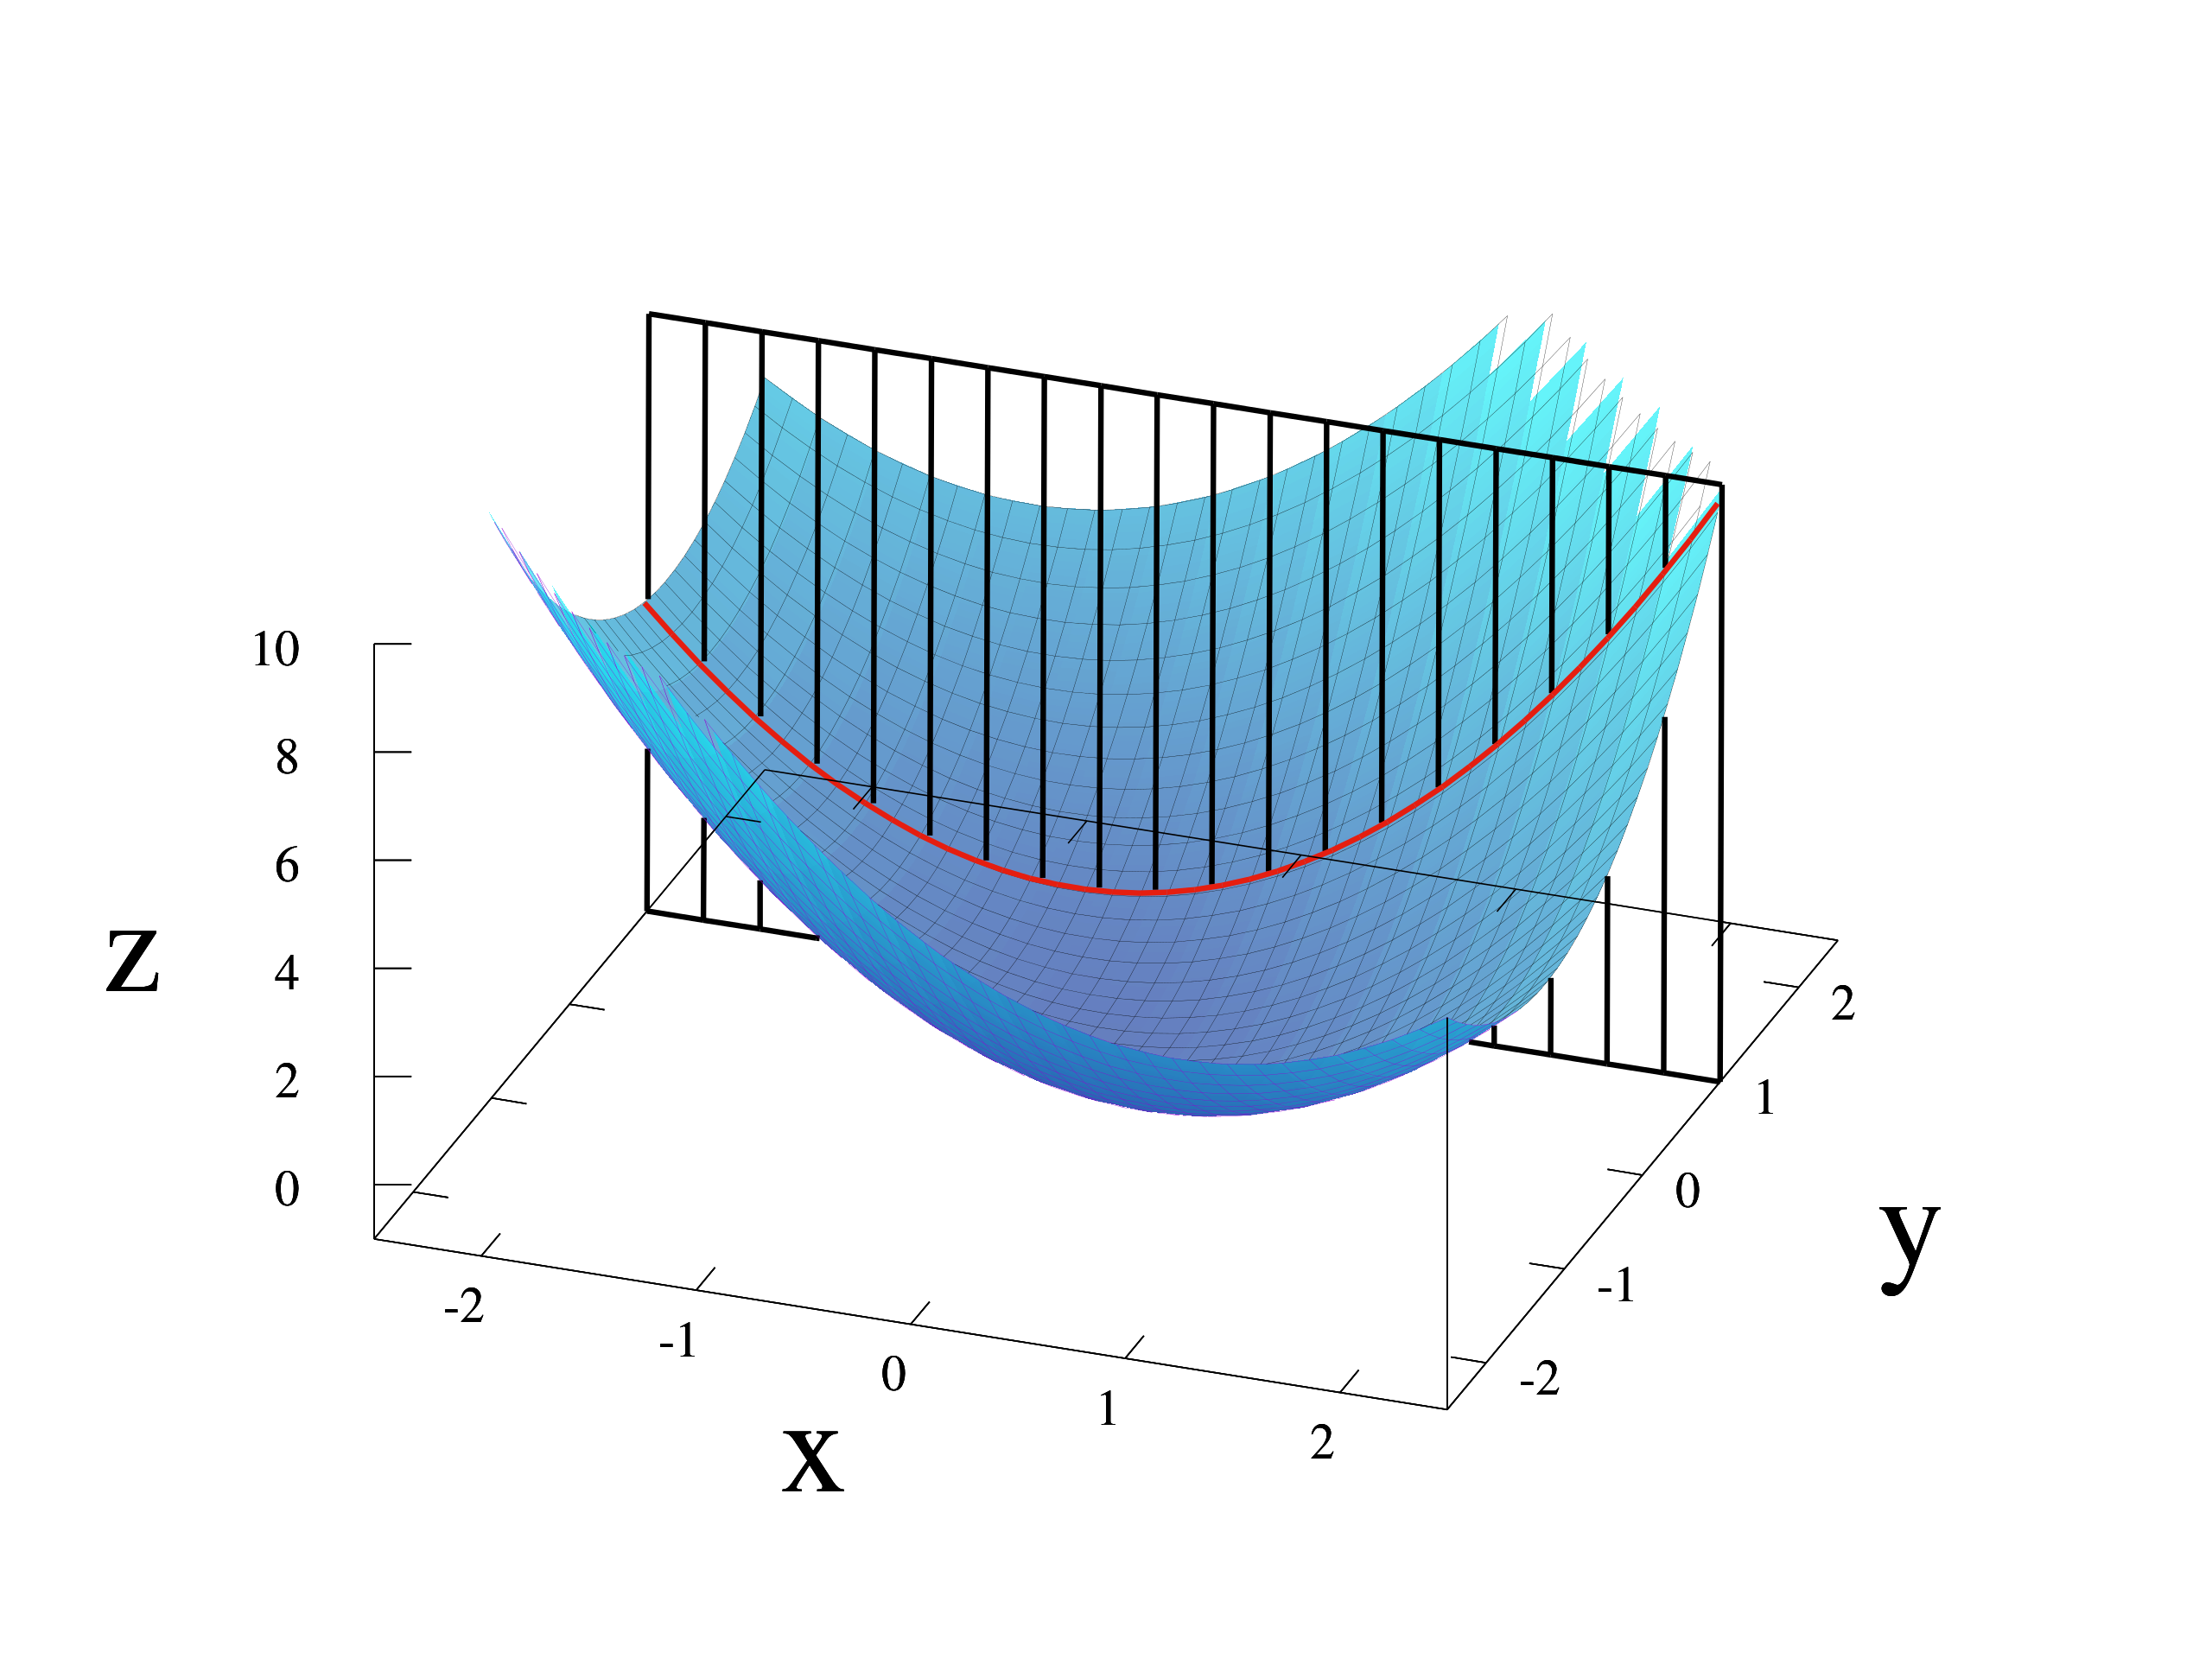
\includegraphics[width=\linewidth]{figs/Partial_func_eg.png}
  \caption{A graph of $z = x^2 + xy + y^2$, as well as the curve
  $z=x^2+x+1$ that results from fixing $y=1$.
  Image taken from Wikipedia~\cite{wiki:partial_derivative}.}
  \label{fig:partial_derivative}
\end{figure}

One can do the same thing holding $x$ fixed and taking a derivative
w.r.t. $y$; this procedure similarly defines a partial derivative w.r.t. 
$y$, $\partial_y f$.
We can generalize this to an arbitrary number of independent variables. 
For example for functions defined in four dimensions, we have a
function $f:\R^4\to\R$ of variables $x_1$, $x_2$, $x_3$, and $x_4$, which we
sometimes indicate\footnote{Similarly a function with a 3-$d$
domain may be indicated as $f(\vec{x})$.} as $f(\fvec{x})$. We define a 
function\footnote{This is simply abstracting our previous equation
\equatref{eq:fixG}. It is saying there is some
equation $g(x_\mu)$ ($\mu$ being one of $x_1$, $x_2$, $x_3$ or $x_4$) which is
equal to some more general equation $f(\fvec{x})$ where in $f(\fvec{x})$ the
variable $x_nu$ is held constant ($\nu$ being one of $x_1$, $x_2$, $x_3$, or
$x_4$ but it can't be the same as $\mu$).}
$g$
\begin{equation}
g(x_\mu)\equiv f(\fvec{x})\,
\suchthat\text{ $x_\nu$ is held constant $\Forall \nu\neq \mu$}
\end{equation}
where $1\leq\mu,\nu\leq4$. 
Then the partial derivative is
\begin{equation}
\pdv{f(\fvec{x})}{x_\mu}=\frac{\dd g(x_\mu)}{\dd x_\mu}.
\end{equation}
For shorthand, we use $\partial_\mu f$.

One further generalization to be made is to allow $f$ to map to a set besides
$\R$. For instance $f$ could be {\it vector-valued}\index{vector-valued} 
or {\it matrix-valued}\index{matrix-valued}, i.e. $f$ could output
vectors or matrices. 
%This can introduce some subtleties, and one may have to be even more careful. 
We won't
discuss these generalizations in these notes, but I just want you to know they
are possible and you will see them eventually.

Next let's discuss multiple integration. Again we start with a simple, 2-$d$
example. Suppose you have two integrable functions $f,g:\R\to\R$. Then by the
fundamental theorem of calculus, you know that when $a\leq x\leq b$.
\begin{equation}\label{eq:2dsimple}
\int_a^b\dd{x}f(x)=F(b)-F(a)~~~~\text{and}~~~~
\int_a^b\dd{x}g(x)=G(b)-G(a)
\end{equation}
for some functions $F$ and $G$, usually called {\it
primitives}\index{primitive}. Now imagine you encounter the product
\begin{equation}\label{eq:2dsimpleEval}
\int_a^b\dd{x}f(x)\int_a^b\dd{y}g(y).
\end{equation}
According to \equatref{eq:2dsimple}, this evaluates to
\begin{equation}
\left(F(b)-F(a)\right)\left(G(b)-G(a)\right).
\end{equation}
There, you just did you first 2-$d$ integral.

You may have noticed that I switched the variable name for $g$ from $x$ in
\equatref{eq:2dsimple} to $y$ in \eqref{eq:2dsimpleEval}. This is because in the
product, I want to notationally emphasize that the integrals are being evaluated
independently. This is no different from when wants to multiply two sums
\begin{equation}
  \sum_{i=1}^n f_i~~~~\text{and}~~~~\sum_{i=1}^n g_i.
\end{equation}
In order to keep track of the fact that the sums run over independent indices,
one writes the product\footnote{Sometimes we use the shorthand
$\sum_{i,j=1}^n$.} as
\begin{equation}
  \sum_{i=1}^n\sum_{j=1}^n f_ig_j.
\end{equation}
The product of integrals is no different, which makes sense if you think about
it since the integrals come from a limiting procedure starting with Riemann
sums. As long as the integration bounds are finite, we can utilize the fact
the order of symbols in the sum can be reorganized to reorganize symbols in the
integral. Hence \equatref{eq:2dsimpleEval} can be written as
\begin{equation}\label{eq:2dprodInt}
\int_a^b\int_a^b\dd{x}\dd{y}f(x)g(y)
=\int_a^b\int_a^b\dd{x}\dd{y}h(x,y),
\end{equation}
where $h(x,y)\equiv f(x)g(y)$. This logic is exactly how one can take the
integral of any function $h(x,y)$ in two dimensions, provided that $h$ can be
factorized into two functions $f$ and $g$ like that. 

%Said another way, we can
%express a function $h(x,y)$ as the product of the functions $f(x)$ and $g(y)$,
%i.e., $h(x,y) = f(x)g(y)$, then we can use the product rule of integration to
%evaluate the double integral of $h(x,y)$ over a region in the $x-y$ plane. The
%product rule of integration states that the double integral of a product of two
%functions $f(x)$ and $g(y)$ over a region $[a,b]\times[c,d]$ can be computed by
%integrating $f(x)$ over $[a,b]$ and $g(y)$ over $[c,d]$, and then multiplying
%the two results together. This is exactly what is done in Equation
%\eqref{eq:2dprodInt}, where we first integrate $f(x)g(y)$ with respect to $x$
%over the interval $[a,b]$, and then integrate the result with respect to $y$
%again over the interval $[a,b]$. This method can be used to evaluate the
%integral of function $h(x,y)$ that can be factorized into $f(x)$ and $g(y)$ like
%$h(x,y) = f(x)g(y)$.

% DC: I commented this out 1) because I'm not sure what is meant by "product rule
% of integration" and 2) because the rest is mostly a restating where the
% language isn't different enough to warrant repeating. I think the main issue
% is that I am not really describing multiple integration well, but I really
% want to avoid to get into the details on this, which will take quite a bit of
% space. I just want the reader to have a vague idea what I mean when I use a
% multiple-integral symbol, and nothing more. Maybe in a future edition I will
% set aside 10 or so pages to do treat it better.

Please note that in the general case, evaluating integrals 2-$d$ functions
is not quite that straightforward! Again, that above prescription only works
when $h$ can be factorized into two functions $f$ and $g$ of $x$ only and $y$
only. For instance it works when $h(x,y)=x^2\sin(y)$.
A function $h_{\text{tricky}}(x,y)=\sin(xy)$ will not integrate as a simple
product.
For now, I just want you to have some vague intuition what multiple integration
means, at least in some cases.
I foist the proper treatment of the general case of 2-$d$
integration onto your multivariable calculus professor.


The above procedure can be generalized to an arbitrary number of variables, as with
the partial derivative. In four dimensions, one encounters integrals like
\begin{equation}
\int_a^b\int_a^b\int_a^b\int_a^b
\dd{x_4}\dd{x_3}\dd{x_2}\dd{x_1}f(\fvec{x}).
\end{equation}
If at some point during the discussion we don't really care about the limits of
integration, we might write
\begin{equation}
\int\dd[4]{x}f(\fvec{x}),
\end{equation}
and if we want to limit the integration domain to some region $R$, for example a
hypersphere or something, we write
\begin{equation}
\int_R\dd[4]{x}f(\fvec{x}).
\end{equation}
Again, this business of shuffling around pieces of the integrand works if
it can be factorized into functions that each depend on one of the integration
variables only.
I just want you to have some intuition what is meant when a multiple integral
symbol appears.

\section{Probability and error}\label{sec:probAndError}

Crucial to the study of quantum physics, statistical physics, experiment, and
eventually lattice field theory is an understanding of probability and the
ability to understand statistics. These skills are actually quite important to
understand all modern science, not just physics, as well as in everyday
circumstances like politics\footnote{In this latter case it is of utmost
importance to understand these subjects to protect oneself against
misinformation. As Benjamin Disareli allegedly once said, ``There are lies,
damned lies, and statistics."}.
You already have a rough idea of probability: It's a way of saying whether you
think something will happen or not, while in general signaling that you aren't
completely certain. We will now make these ideas precise.

We will consider a {\it random variable}\index{random variable}\footnote{In this
section I will try to denote random variables by capital letters.} $X$ which
has some possible {\it outcomes}\index{outcome} $x_i$. The random variable will take 
one of the values in $x_i$, but we don't know for sure which one.
The set of all possible outcomes
\begin{equation}
  \Omega=\{x_1,x_2,...,x_N\},
\end{equation}
assuming there are $N\in\N$ possible outcomes, is called the {\it sample
space}\index{sample space}. If $|\Omega|$ is finite as in the above case, we
say that $X$ is {\it discrete}\index{discrete}. An {\it event}\index{event} $E$
is any subset of outcomes $E\subset\Omega$, and we assign it a {\it
probability}\index{probability} $\pr{E}$. Axiomatically speaking, the
probability has to fulfill two conditions:
\begin{enumerate}
  \item $\Forall E$, $0\leq\pr{E}\leq1$.
  \item $\pr{\Omega}=1$, i.e. the random variable $X$ needs to have some outcome
in $\Omega$. Another way to state this is that the probability of at least one
of the possibilities is 1. 
\end{enumerate}

Pragmatically you can assign a probability by repeating some experiment $n$
times. If the event $E$ occurs $N_E$ times, then
\begin{equation}
  \pr{E}\equiv\lim_{N\to\infty}\frac{N_E}{N}.
\end{equation}
Alternative, you can make some theoretical assignment of probabilities to
events. For instance when one tosses a coin, if one has no reason to believe the
coin is biased, it must be that
\begin{equation}
\pr{\text{heads}}=\pr{\text{tails}}=\frac{1}{2}.
\end{equation}
This theoretical assignment is nice, but it should eventually be checked against
some observation or measurement as well.

To be quantitative, we like to somehow map the possible outcomes to numbers. For
instance a die roll can be mapped to the set $\{1,2,3,4,5,6\}$. A reasonable
question to ask in this case is: If I toss a die, what can I expect? A measure
of this is the {\it expectation value}\index{expectation value}, which is
defined by
\begin{equation}
\ev{X}=\sum_{x\in\Omega}\pr{X=x}x,
\end{equation}
or more explicitly for the die,
\begin{equation}
\ev{\text{my die roll}}=\sum_{i=1}^6\frac{1}{6}\,i=3.5.
\end{equation}

Sometimes the cardinality of $\Omega$ is uncountably infinite. For instance you
may ask something like: What is the probability that a particle in this gas has
a speed between $v_1$ and $v_2$? In this case, the sample space is
\begin{equation}
  \Omega=\{x\suchthat0\leq x\leq c\},
\end{equation}
where $c$ is the speed of light\footnote{As we will reiterate in
\secref{sec:SR}, $c$ is the largest possible speed for anything.}.
In such a case we speak of a {\it continuous} random variable $X$.
The probability that $X$ takes any one particular value in $\Omega$ is
zero\footnote{Intuitively you could ask yourself: What is the probability that
my speed is exactly $\pi$ to all infinitely many digits? When checking against
experiment, you will never be able to resolve all infinitely many digits, so at
best you must specify a range corresponding to the resolution of your
instrument. In formal mathematical language, we require $\Omega$ to be
{\it measurable}.}. 
We can only assign
sensible probabilities to subsets of $\Omega$ of uncountably infinite
cardinality. In the above
case, this corresponds to the range of velocities between $v_1$ and $v_2$.
The probability that $X$ takes a value in the small range of velocities $\dd x$
is denoted
\begin{equation}
   \pr{X\in[x,x+\dd x]}=\dd{x}f(x),
\end{equation}
and hence for continuous random variables, the probability must instead
fulfill the properties
\begin{enumerate}
  \item  $0\leq\dd{x}f(x)\leq 1$ and
  \item $\int_{x\in\Omega}\dd{x}f(x)=1$.
\end{enumerate}
We call $f$ the {\it probability density function}\index{probability density
function} or PDF.
Correspondingly, the notion of an expectation value\index{expectation value}
must change as
\begin{equation}
\ev{X}=\int_{x\in\Omega}\dd{x}f(x)\,x.
\end{equation}
Meanwhile the {\it cumulative distribution function} (CDF) is the function
\index{CDF}
$F(x)$ given by
\begin{equation}
  F(x)\equiv \pr{X<x}=\int_{-\infty}^x\dd{t}f(t).
\end{equation} 



\begin{example*}{}{}
Two examples of important probability distributions include the {\it Gaussian}
or {\it normal} distribution,\index{PDF!normal}
\begin{equation}
  \gau(x,\hat{x},\sigma)\equiv\frac{1}{\sigma\sqrt{2\pi}}
  \exp\Bigg(-\frac{(x-\hat{x})^2}{2\sigma^2}\Bigg)
\end{equation}
where $\sigma$ is the standard deviation of the distribution and $\hat{x}$ is
the mean, and the {\it Cauchy} \index{PDF!Cauchy} distribution,
\begin{equation}
  \cau(x,\alpha)\equiv\frac{\alpha}{\pi\big(\alpha^2+x^2\big)}.
\end{equation}
I will refer to these special PDFs later, particularly the normal distribution.
I'll call their CDFs $\Gau$ and $\Cau$, respectively.
\end{example*}

From now on, we consider continuous random variables only.
Now that we know what probabilities and PDFs are, we can start thinking about
ways to characterize them. For example we can think about typical values taken
by a random variable from some distribution. We can get some information
from the mean and variance of a distribution. These are
both special cases of a more general concept.
In particular, let $n\in\N$.
  The {\it $n\nth$ moment} \index{moment}of the distribution $f(x)$ is
  \begin{equation}\label{dfn:mom}
    \ev{X^n}=\int_{-\infty}^\infty\dd{x}x^nf(x).
  \end{equation}

The mean and variance are the special cases $\hat{x}=\ev{X}$ and
$\sigma^2=\ev{(X-\hat{x})^2}$. Sometimes we call the mean the {\it expected
value}\index{expected value} or {\it expectation value}\index{expectation
value}, and sometimes we denote the variance $\variance$. Note that not all
probability distributions have well-defined moments. The Cauchy distribution is
very ill-behaved in this regard, since its $n\nth$ moment diverges
$\Forall n\in\N$.
Generally in the lab, one draws random variables from distributions
about which one has no a priori knowledge. Therefore in principle one
doesn't know the true moments these distributions. The
definition \eqref{dfn:mom} suggests a way to estimate them.
Suppose you draw a sample $X_1,...,X_N$:
  An {\it estimator}\index{estimator} of the $n\nth$ moment, $n\in\N$, is
  \begin{equation}
    \bar{X}^n\equiv\frac{1}{N}\sum_{i=1}^N X_i^n.
  \end{equation}
In the case $n=1$ we obtain the ordinary arithmetic average.
We use the hat to distinguish true values from estimators, which will
generally be denoted with a bar. For estimators of moments besides the
mean, we must be more careful.

Consider two intervals $[a,b]$ and $[c,d]$ and two random variables
$X$ and $Y$ drawn from PDFs $f$ and $g$, respectively. Then $X$ and $Y$ are
said to be {\it independent}\index{random variable!independent} if
\begin{equation}\label{dfn:ind}
  \pr{X\in[a,b]\text{ and }Y\in[c,d]}=\int_a^b\int_c^d\dd{x}\dd{y}f(x)\,g(y)
\end{equation}
Hence we see that the {\it joint PDF}\index{PDF!joint} of $X$ and $Y$
is $f(x)g(y)$. On the other hand, we say $X$ and $Y$ are {\it uncorrelated}
\index{random variable!uncorrelated} if
\begin{equation}
  \ev{XY}=\ev{X}\ev{Y},
\end{equation}
The {\it covariance}\index{covariance}
\begin{equation}\label{dfn:cov}
  \Cov[X,Y]\equiv\ev{XY}-\ev{X}\ev{Y}
\end{equation}
can be used to give a measure of how correlated $X$ and $Y$ are, or
one can use the {\it correlation}\index{correlation}
\begin{equation}\label{dfn:cor}
  \rho(X,Y)=\frac{\Cov[X,Y]}{\sqrt{\sigma^2_X\sigma^2_Y}}.
\end{equation}
So equivalently we say $X$ and $Y$ are correlated if $\rho(X,Y)=0$.
It's worth emphasizing that if $X$ and $Y$ are independent,
it follows that they are uncorrelated. This can be seen by applying
definition \eqref{dfn:mom} to the random variable $XY$, then using
definition \eqref{dfn:ind}. However if $X$ and $Y$ are
uncorrelated, {\it they can still be dependent}.
\begin{example*}{}{}
  Here's an extreme example by Cosma Shalizi~\cite{cosma_indep}.
Let $X$ be uniformly distributed
  on [-1,1] and let $Y=|X|$. Then clearly $Y$ depends on $X$. However it
  is easy to see that $Y$ is uniform on [0,1] and $\ev{XY}=0=\ev{X}\ev{Y}$.
  Hence $X$ and $Y$ are not correlated.
\end{example*}

The next two propositions show us how to add expectation values and
random variables. Let $X$ and $Y$ be independent random variables
drawn from PDFs $f$ and $g$, respectively.
\begin{proposition}{}{}
  Let $a,b\in\R$ be constants. Then
  $$\ev{aX+bY}=a\ev{X}+b\ev{Y}.$$
  \begin{proof}
    Since $X$ and $Y$ are independent, their joint PDF is $fg$. Then
    \begin{equation*}
      \begin{aligned} 
      \ev{aX+bY}&=\int\dd{x}\dd{y}(ax+by)f(x)g(y)\\
                &=a\int\dd{x}\dd{y}x\,f(x)g(y)+
                 b\int\dd{x}\dd{y}y\,f(x)g(y)\\
                &=a\int\dd{x}x\,f(x)+b\int\dd{y}y\,g(y)\\
                &=a\ev{X}+b\ev{Y}.
      \end{aligned}
    \end{equation*}
  \end{proof}
\end{proposition}

\begin{proposition}{}{addvars}
  The PDF of the random variable $Z=X+Y$ is given by the convolution
  \begin{equation*}
    h(z)=\int_{-\infty}^\infty\dd{x}f(x)g(z-x)
  \end{equation*}
  \begin{proof}
    The CDF of $Y$ is, according to \equatref{dfn:ind},
    \begin{equation*}
      H(y)=\int_{x+y\leq z}\dd{x}\dd{y}f(x)g(y)
          =\int_{-\infty}^\infty\dd{x}f(x)\int_{-\infty}^{z-x}
            \dd{y}g(y).
    \end{equation*}
    The PDF $h$ follows from the Fundamental Theorem of Calculus:
    \begin{equation*}
      h(z)=\dv{H}{z}=\dv{H}{(z-x)}
          =\int_{-\infty}^\infty\dd{x}f(x)g(z-x).
    \end{equation*}
  \end{proof}
\end{proposition}


\subsection{The normal distribution}
\index{PDF!normal}
Now we're going to focus on results about the normal distribution specifically.
This first proposition will aid us in some of the calculations.

\begin{proposition}{}{gauss}
  Let $\alpha>0$. Then
  \begin{equation*}
    \int_{-\infty}^\infty\dd{x}e^{-\alpha x^2}=\sqrt{\frac{\pi}{\alpha}}.
  \end{equation*}
  \begin{proof}
    The trick is to just square the LHS:
    \begin{equation*}\begin{aligned}
      \left(\int_{-\infty}^\infty\dd{x}e^{-\alpha x^2}\right)^2
      &=\int_{-\infty}^\infty\int_{-\infty}^\infty\dd{x}\dd{y}
        e^{-\alpha(x^2+y^2)}\\
      &=\int_0^\infty \dd{r}r\int_0^{2\pi}\dd{\theta}e^{-\alpha r^2}\\
      &=\frac{\pi}{\alpha}.
    \end{aligned}\end{equation*}
  \end{proof}
\end{proposition}

For the next result
let $X_1$ and $X_2$ be two independent random variables drawn from normal
distributions with respective means $\hat{x}_1$ and $\hat{x}_2$ and
standard deviations $\sigma_1$ and $\sigma_2$.
\begin{proposition}{}{addgauss}
  The random variable $Y=X_1+X_2$ is normally distributed with mean
  $\hat{x}_1+\hat{x}_2$ and variance $\sigma_1^2+\sigma_2^2$.
  \begin{proof}
    By \propref{prp:addvars}, the sum $Y$ has the distribution
    \begin{equation*}
      g(y)=\frac{1}{2\pi\sigma_1\sigma_2}
           \int_{-\infty}^\infty\dd{x}\exp\left[
             -\frac{(x-\hat{x}_1)^2}{2\sigma_1^2}
             -\frac{(y-x-\hat{x}_2)^2}{2\sigma_2^2}\right].
    \end{equation*}
    Pull everything out of the integral that doesn't depend on $x$,
    then complete the square with what's left over.
    One obtains for $g(y)$
    $$
      \frac{1}{2\pi\sigma_1\sigma_2}
           \exp\left[-\frac{(y-\hat{x}_1-\hat{x}_2)^2}
                      {2(\sigma_1^2+\sigma_2^2)}\right]
           \int_{-\infty}^\infty\dd{x}
           \exp\left[-\frac{\sigma_1^2+\sigma_2^2}
                     {2\sigma_1^2\sigma_2^2}(x+C)^2\right],
    $$
    where $C$ is just a bunch of stuff that doesn't depend on $x$.
    Therefore you can make the substitution $u=x+C$ with $\dd u=\dd x$ and
    carry out the new integral using \propref{prp:gauss}.
    The result is
    \begin{equation*}
      g(y)=\frac{1}{\sqrt{2\pi(\sigma_1^2+\sigma_2^2)}}
           \exp\left[-\frac{(y-\hat{x}_1-\hat{x}_2)^2}
                      {2(\sigma_1^2+\sigma_2^2)}\right].
    \end{equation*}
  \end{proof}
\end{proposition}

Since the normal distribution is so important, so must be its CDF.
Unfortunately the integral of the normal PDF is {\it non-elementary};
\index{non-elementary} that is, it can't be expressed in terms of
polynomials or standard
functions like $\sin$, $\cos$, or $\exp$. Therefore we give a name
to this special function.
The {\it error function}\index{error function} is
\begin{equation}
  \erf(x)\equiv\frac{2}{\sqrt{\pi}}\int_0^x\dd{t}e^{-t^2}.
\end{equation}
Then we can write the Gaussian CDF with mean 0 as
\begin{equation}
  \label{eq:gaussCDF}
  \Gau(x,0,\sigma)=\frac{1}{\sqrt{2\pi}\sigma}
                   \int_{-\infty}^x\dd{t}e^{-t^2/2\sigma^2}
                  =\frac{1}{2}+\frac{1}{2}
                   \erf\left(\frac{x}{\sqrt{2}\sigma}\right).
\end{equation}
Now we can list some pretty powerful applications of the normal distribution.
For instance one often must compare two empirical estimates of some mean.
Usually these estimates are different, and one might wonder whether this
disparity is real or just plain unlucky. More precisely:
\index{Gaussian difference test}
\begin{theorem}{Gaussian difference test}{}\label{thm:gaudif}
  Suppose $\bar{X}$ and $\bar{Y}$ are correct estimates of
  some expectation
  value, i.e. they are normally distributed with the same mean, and call
  their respective standard deviations $\sigma_X$ and
  $\sigma_Y$. Then the probability that $\bar{X}$
  and $\bar{Y}$ differ by at least $D$ is
  \begin{equation*}
    \pr{|\,\bar{X}-\bar{Y}|>D}=1-\erf\left(\frac{D}
       {\sqrt{2(\sigma_X^2+\sigma_Y^2)}}\right).
  \end{equation*}
  \begin{proof}
    From \propref{prp:addgauss}, the random variable
    $\bar{X}-\bar{Y}$ is normally distributed with mean 0
    and variance $\sigma_D^2=\sigma_X^2+\sigma_Y^2$. Therefore by
    \equatref{eq:gaussCDF}, the probability that $\bar{X}$ and
    $\bar{Y}$ are at most $D$ apart is
    \begin{equation*}
      \begin{aligned}
        \pr{|\,\bar{X}-\bar{Y}|<D}
            &=\pr{-D<\bar{X}-\bar{Y}<D}\\
            &=\Gau(D,0,\sigma_D)-\Gau(-D,0,\sigma_D)\\
            &=1-2\Gau(-D,0,\sigma_D)\\
            &=\erf\left(\frac{D}{\sqrt{2}\sigma_D}\right).
      \end{aligned}
    \end{equation*}
    And of course, $\pr{|\,\bar{X}-\bar{Y}|>D}
     =1-\pr{|\,\bar{X}-\bar{Y}|<D}$.
  \end{proof}
\end{theorem}
In other words, the above theorem gives the probability that the
observed difference $|\bar{X}-\bar{Y}|$ is due to chance. This probability
is called the \index{q-value}{\it q-value}. In practice one sets some
threshold on $q$ below which one investigates further whether the
underlying distributions of the estimates are different. Often one
takes the threshold as 0.05.

Finally, suppose you're an experimenter taking independent measurements of
some observable. Furthermore suppose you don't know anything about the
observable, except that it comes from some distribution with finite variance.
The central limit theorem (CLT) says that armed with this information alone,
you know that the sample mean will be normally distributed about
the true mean. Here is the precise statement.\index{Central limit theorem}
\begin{theorem}{Central limit theorem}{}
  Let $X_1,...,X_N$ be $N$ independent random variables drawn from PDF $f$.
  Suppose further that $f$ has mean $\hat{x}$ and variance $\sigma^2$.
  Then the PDF of the estimator $\bar{X}$ converges to
  $\gau(\bar{X},\hat{x},\sigma/\sqrt{N})$.
\end{theorem}
The only proof of this theorem I'm aware of requires the introduction of
{\it characteristic functions}, which I would like to avoid. So I will ask you
to trust this theorem. The central limit theorem tells you that, if you have
some experiment you repeat $N$ times, the arithmetic mean $\bar{X}$ is likely to
be only $\sigma/\sqrt{N}$ away from the true mean $\hat{x}$. As you increase
$N$, this statement becomes more tight, which corresponds to the intuition that
as you repeat an experiment more and more times, you have a more and more exact
understanding of things.
More specifically, for large enough $N$, we expect the true mean to be within
$\sigma/\sqrt{N}$ of the estimator roughly 68\% of the time.
\tabref{tab:normal} gives the area under a Gaussian curve
for different numbers of standard deviations away from the mean.

\begin{table}
\centering
\caption{Table of areas under the curve for the normal distribution.
The last column gives the probability that a random variable
drawn from the distribution falls at least the given number of error bars
away from the mean.}
\begin{tabularx}{\linewidth}{cCr}
\hline\hline
Number of $\sigma$ from $\hat{x}$ & Area under curve & About 1 in ...\\
\hline
1 & 0.682 689 49 & 3\\
2 & 0.954 499 74 & 22\\
3 & 0.997 300 20 & 370\\
4 & 0.999 936 66 & 15 787\\
5 & 0.999 999 43 & 1 744 278\\
\hline\hline
\end{tabularx}
\label{tab:normal}
\end{table}


\section{Bias}\label{sec:bias} 

For this section consider independent random variables $X_1,...,X_N$ 
drawn from a distribution with mean $\hat{x}$ and variance $\sigma^2$.
Earlier we recovered the familiar estimator for the mean, which was
just the ordinary arithmetic average. But what about an estimator for
the variance? Naively one might write
\begin{equation}\label{eq:bad}
  \bar{\sigma}^2_{\text{biased}}=\frac{1}{N}\sum_{i=1}^N(X_i-\bar{X})^2;
\end{equation} 
While we expect this estimator to converge\footnote{An estimator that
converges to the correct result as $N\to\infty$ is 
{\it consistent}\index{consistent}. Note that unbiased and consistent
do not mean the same thing; in particular $\bar{\sigma}^2_{\text{biased}}$
is consistent but biased.} to the
exact result in the limit $N\to\infty$, it disagrees with
$\sigma^2$ for small $N$. Most glaringly when $N=1$, the
estimator is zero, regardless of the exact result. 
\index{bias}
An estimator is said to be {\it biased} when its expectation value
does not agree with the exact result. The difference between the
expectation value of the estimator and the exact result is
correspondingly called the {\it bias}. When they agree, we say
the estimator is {\it unbiased}.
\begin{proposition}{}{stdev}
  An unbiased estimator of the variance is
  $$
    \bar{\sigma}^2=\frac{1}{N-1}\sum_{i=1}^N(X_i-\bar{X})^2.
  $$
  \begin{proof}
  To construct an unbiased estimator of the variance,
  we'll determine the bias of the estimator, then remove it. Note
  \begin{equation*}
    \ev{\bar{\sigma}^2_{\text{biased}}}=\frac{1}{N}\sum\limits_{i=1}^N
      \left(\ev{X_i^2}-2\ev{X_i\bar{X}}+\ev{\bar{X}^2}\right).
  \end{equation*}
  Let us analyze the above equation term by term. Since the random
  variables $X_i$ are drawn from the same distribution, the first term
  is an unbiased estimator of $\ev{X^2}$ for each $i$. Next the
  second term can be rewritten as
  \begin{equation*}
    \begin{aligned}
    \ev{X_i\bar{X}}&=\frac{1}{N}\left(\ev{X_i^2}+
                     \sum_{j\,|\,j\neq i}\ev{X_iX_j}\right)\\
                   &=\frac{1}{N}\left(\ev{X^2}+(N-1)\ev{X}^2\right)\\
                   &=\frac{1}{N}\left(\ev{X^2}-\ev{X}^2\right)+\ev{X}^2\\
                   &=\frac{\sigma^2}{N}+\hat{x}^2,
    \end{aligned}
  \end{equation*}
  where in the second line we used the independence of the $X_i$. Finally
  for the last term we have
  $$
    \ev{\bar{X}^2}=\ev{\frac{1}{N^2}\sum_{i,j}X_iX_j}
        =\frac{1}{N^2}\left(N\ev{X^2}+\sum_{i,j\,|\,i\neq j}\hat{x}^2\right)
        =\frac{\sigma^2}{N}+\hat{x}^2,
  $$
  where we again used independence in the second equality. Plugging
  everything into $\ev{\bar{\sigma}^2_{\text{biased}}}$ gives
  \begin{equation*}
      \ev{\bar{\sigma}^2_{\text{biased}}}
        =\frac{1}{N}\sum_{i=1}^N
          \left(\ev{X^2}-\frac{\sigma^2}{N}-\hat{x}^2\right)
        =\left(\frac{N-1}{N}\right)\sigma^2.
  \end{equation*}
  This equation shows us the bias is $-\sigma^2/N$. Therefore according
  to this equation, an unbiased estimator of the variance is
  $$
    \bar{\sigma}^2=\left(\frac{N}{N-1}\right)\bar{\sigma}_\text{biased}^2
                  =\frac{1}{N-1}\sum_{i=1}^N(X_i-\bar{X})^2
  $$
  as we wished to show.
  \end{proof}
\end{proposition}



\section{Groups}

Very roughly, a group is a set with a rule that lets you combine two group
elements to make a new one. More precisely, 
a {\it binary operation} \index{binary operation} $\bullet$ on a set 
$G$ is a function $\bullet : G\times G\to G$. A {\it group} \index{group}
 is a set $G$ equipped with a binary operation $\bullet$ that satisfies 
the following axioms:
  \begin{enumerate}
    \item $\bullet$ is associative.
    \item $\Exists \id \in G\suchthat\Forall g \in G$, 
          \begin{equation}
            \id\bullet g=g\bullet \id=g. 
          \end{equation} This element $\id$ is called the {\it identity}.
          \index{identity}
    \item $\Forall g \in G,~\Exists g^{-1} \in G$, called the 
          {\it inverse} \index{inverse} of $g$, such that
          \begin{equation}
            g^{-1}\bullet g=g\bullet g^{-1}=\id.
          \end{equation}
  \end{enumerate}
If group elements commute under $\bullet$ the group is said to be
{\it abelian}\index{abelian}. The {\it order} \index{order} of a group, 
denoted $|G|$, is its cardinality. A {\it subgroup} \index{subgroup}
$H$ of $G$ is a non-empty subset of $G$ that itself forms a group under 
$\bullet$ and in this case we will write\footnote{
It should be clear from context whether this symbol indicates group 
organization or magnitude.} 
$H\leq G$. 
%Finally a group is {\it cyclic} \index{cyclic}
%if it is generated by a single element; that is, if 
%$\Exists g\in G$ such that $G=\{g^{n}\suchthat  n\in\Z\}$.

It's not too common to write the
$\bullet$ explicitly when showing the composition of two elements. So for
example you will often see $gh$ as shorthand for $g\bullet h$. In general I will
only refer to operations on algebraic structures explicitly when giving the
definition of that structure. Therefore you can expect to see $gh$ instead of
$g\bullet h$ from here on out.

Here I want to prove a small fact about groups, just to give you an idea of how
such a proof would work. Basic facts about groups don't usually require any
tricks; you can usually just chase definitions.

\begin{proposition}{}{}
  A subset H of G is a subgroup of G if and only if
  $$a,b\in H\Rightarrow ab^{-1}\in H$$
  \begin{proof}
    ($\Rightarrow$) Follows immediately from the definition of a subgroup. To 
    show ($\Leftarrow$) let $b\in H$. Then by the above conditional, $bb^{-1}
    \in H$, which shows $\id\in H$. To show the existence of inverses in $H$, 
    note $\id,b\in H\Rightarrow \id b^{-1}\in H\Rightarrow b^{-1}\in H$. 
    Finally, associativity is inherited from G.
  \end{proof}
\end{proposition}

\begin{example*}{}{}
\begin{enumerate}
  \item $\Z,\ \Q,\ \R$, and $\C$ are all groups
        under addition, and
        $$ 
          \Z \leq \Q \leq \R \leq \C.
        $$ 
        Each of these sets with 0 removed could also form a group under
        multiplication.
  \item Sets of objects besides numbers also form groups. For example let $V$ 
        be any non-empty set of objects and let $S_{V}$ be the set of all
        permutations of $V$. Then $S_{V}$ forms a group under function
        composition called the {\it symmetric group}\index{group!symmetric} 
        on the set $V$.
\end{enumerate}
\end{example*}

\subsection{Why do groups matter in physics?}\label{sec:groupsMatter}

Besides the examples of groups discussed above, one common type of group is a
group of symmetries of some system. For example consider the circle of radius 1. 
All rotations in the plane of the circle are symmetries of the circle. 
Any point on the circle can be represented as a vector
\begin{equation}\label{eq:s}
\vec{s}=\colvec{2}{\cos\theta}{\sin\theta}, 
\end{equation}
where $0\leq\theta<2\pi$. Let
\begin{equation}\label{eq:rot}
R_\phi\equiv\left(\begin{array}{cc}
          \cos\phi   & -\sin\phi  \\
          \sin\phi   &  \cos\phi  \\
            \end{array}\right). 
\end{equation}
This matrix will rotate $\vec{s}$ by an angle $\phi$.
This can be seen by applying $R_\phi$ to $\vec{s}$ using matrix multiplication
and using some trig identities. More importantly the set
\begin{equation}
\U(1)=\{R_\phi\suchthat0\leq\theta<2\pi\}
\end{equation}
forms a group. This is sometimes called the\index{circle group} {\it circle
group} or the\index{unitary group} {\it unitary group of degree 1}\footnote{As
the name suggests, the matrix representation of this group can be shown to be
unitary as defined in \secref{sec:vecmat}.}.

Every finite group can be expressed using matrices.
A set of matrices that behave the same way as a group is called
a\index{matrix representation} {\it matrix representation}. Many infinite groups
also have matrix representations. Matrix representations are often useful to get
some intuition for how a group works. Equation~\eqref{eq:rot} effectively
summarizes a representation of $\U(1)$.

Symmetry groups, especially continuous symmetry groups like $\U(1)$, are of
utmost importance in physics. This was discovered by Emmy Noether in the early
1900s. We give a rough\footnote{I use the word ``system" here in an
intentionally vague way. The correct statement requires to introduce the {\it
action} of a system; then one is rather interested in symmetries of the action.
You will learn more about this as you continue in physics. I view this
discussion as too much detail for a first interaction with LFT.} 
statement of her theorem without proof, which again would
be a bit too much of a digression.
\begin{theorem}{Noether}{}
For every continuous symmetry of a system, there exists a corresponding 
conserved quantity.
\end{theorem}

The conserved quantity in Noether's theorem is called a\index{charge} {\it charge}.
This name is chosen purposefully: from the modern perspective of particle
physics, the electric charge is closely connected with the group $\U(1)$. 
Moreover a class of elementary particles, the so-called\index{boson} 
{\it gauge bosons}, are thought to be, in a sense, physical manifestations of
these symmetries. This suggests that the idea of a charge is more general than
just electric charge, and that other groups may correspond to other charges and
particles.


\subsection{Which groups will we care about?}

We are going to eventually investigate quantum chromodynamics (QCD), which describes
one corner of particle physics. There we will encounter a new charge called
{\it color}\footnote{Here the word color is used as an analogy. It has nothing
to do with visible light.}, and its corresponding symmetry group is the
{\it special unitary group of degree $N_c$}, $\SU(N_c)$, where $N_c$ is the number of
colors. In nature $N_c=3$, but it is sometimes of academic interest to consider
different numbers of colors.

The fact that $N_c=3$ is actually what led to the use of the
terminology\index{charge!color} ``color charge". Let's try to understand this. 
In electromagnetism (EM), there is only one kind of charge,
the\index{charge!electric} electric charge. It can be positive or negative. If I
would like to make an electric-charge-neutral state, I can accomplish this only
by adding as many positive charges as negative charges.
In QCD, there are three kinds of charges, which we sometimes call {\it red},
{\it green}, and {\it blue}. If I have a system with three particles, each
having respectively red, green, and blue color charge, I get a 
color-charge-neutral state. This color naming is thus a mnemonic, for if I mix
red, green, and blue paint, I get white paint.

So $\SU(3)$ will be the group we care about the most. Associated to this
symmetry group is, according to Noether, a conserved charge. This is the color
charge. The particle that we consider a physical manifestation of this symmetry
is the\index{gluon} {\it gluon}. The gluon is responsible for mediating one of
the fundamental forces, which we will discuss in more detail in \secref{sec:SM}.

\section{Further reading}

I have given an extremely superficial introduction to most of these subjects. If
you would like some additional resources, besides taking classes, I can suggest
a few books I found useful.
\begin{itemize}
  \item Rigorous single-variable calculus: 
{\it Calculus} by Michael Spivak~\cite{spivak08} is probably the best
introduction to real analysis that I have tried.
Rubin's {\it Principles of Mathematical Analysis}~\cite{rudin1976principles} is
at a much higher level and less pedagogical, but it does contain a construction
of $\R$ from $\Q$.
  \item Multivariable calculus: For doing practical calculations in one or more
variables I found 
{\it Calculus with Analytic Geometry} by Simmons~\cite{simmons1995calculus}
to be quite helpful.
  \item Linear algebra: Curtis's
{\it Linear Algebra: An Introductory Approach} is quite rigorous, but perhaps
not particularly helpful in building intuition. It's the only book I've tried. 
  \item Probability: I found
Feller's {\it An Introduction to Probability Theory and Its 
Applications}~\cite{feller1}
to be rigorous, readable, and full of fun problems.
  \item Group theory:
If you would like to understand group theory more deeply,
a really good, rigorous introduction to groups accessible to undergrads is 
Dummit and Foote~\cite{dummit_abstract_2004}. To learn about Lie groups
like $\SU(3)$, my personal favorite resource is Georgi~\cite{georgi_lie_1999}.
\end{itemize}
There are also books that try to capture large swathes of math methods in
physics. Probably the most popular is Arfken's {\it Mathematical Methods for
Physicists}~\cite{garfken67:math}.

\section*{Exercises}

\begin{enumerate} 
  \item Let $n\in\N$. Prove that vectors in $\R^n$ are associative, commutative,
        and distributive.
  \item Prove that $\id_n M=M$ for any $n\times n$ matrix $M$.
  \item If $M$ is invertible, will it commute with its inverse? Why or why not?
  \item Prove that $\Q$, $\R$, and $\C$ form groups under addition. Also
        prove it for multiplication.
  \item Show that $R_\phi$ defined in \equatref{eq:rot} rotates $\vec{s}$ defined
        in \equatref{eq:s} by $\phi$. {\it Hint}: You will eventually use some
        trigonometry identities.
  \item Show that $R_\phi$ is a unitary matrix.
  \item Prove that $\U(1)$ is a group.
\end{enumerate}


\bibliographystyle{unsrtnat}
\bibliography{bibliography}
 

\chapter{Some physics}\label{ch:physics}



When I was an undergrad, I majored in both math and physics. Through my math
major I learned some useful things about how mathematical structures work on a
fundamental level. However I think my math major was detrimental to my
understanding of physics philosophy. In math, you start with some rules or {\it
axioms}, and {\it formally derive} everything from that using logic only. 
These derivations are organized as proofs. I found it pretty satisfying to 
come to the end of a proof, because I felt like I had some airtight, undeniable 
knowledge about something. 

Physics is not really the same, in that physicists will often 
use facts that cannot be derived in that way. These facts come from
observing the world, which is usually accomplished via experiments.
For instance, the laws that govern electrodynamics, {\it Maxwell's equations},
are known through observation. More sophisticated theories from which one
can ``derive" Maxwell's equations {\it were tailored in part to achieve that
end}. If you think about it this makes sense: If you already know that Maxwell's
equations are true, then if you want to make a more sophisticated theory, you
better at least recover Maxwell's equations. 
Comparison of our ideas with experiment is viewed as the ultimate check.

Let me introduce some terminology. By {\it model}, I will mean roughly ``the
ideas we have about how the world works." A model is just a way of thinking
about reality. There is nothing that forbids two models from describing the same
reality\footnote{Provided that the models don't contradict each other in some
way.}. Models have observations at their foundation, and they are extended using
logic and sometimes assumptions. Sometimes these extensions will tell you
something quantitative about a natural phenomenon that you are not currently
observing or a phenomenon that has not yet been observed: this is a {\it
prediction}. If a prediction agrees with experiment, it lends credence to our
model, and by extension to our assumptions, if we made any.
In my view, {\it models are not any more real than that}. 
They are a faithful description of reality exactly to the extent that they 
agree with observations and yield correct experimental results.

That may make you feel uncomfortable or feel ambiguous, but I find it
empowering. First of all at least in physics, accepted models yield extremely
precise precisions that turn out to be accurate. Secondly, it gives physicists
some leeway when developing and understanding their models. We are free
to use assumptions that will make our calculations easier, and we are free to
think about reality however we like, {\it as long as we ultimately obtain quantitative
results that agree with experiment, and as long as our models are free of
contradictions}.

In the following, I am going to introduce some basic ideas in physics that I
think are necessary to have some understanding of lattice field theory.
Some of these ideas about reality may seem
counterintuitive, uncomfortable, or bizarre. Nevertheless, these ideas, these
ways of thinking about things, seem to be correct, again because they eventually
produce highly precise quantitative predictions that are vindicated in
experiment time and time again. 


\section{Units and dimensional analysis}


Measurements have units, and therefore units are of fundamental importance when 
interpreting things in physics. They are so important, that I like to set them off 
with square brackets []. For instance all distances can be measured in [mi] (miles), 
all times in [h] (hours), all weights in [lb] (pounds), and so on. 
Besides connecting numbers to the natural world, units are an opportunity to
check for errors. Once you have settled on a {\it unit system}, which I will
discuss more in \secref{sec:units}, two guidelines you can use are
\begin{enumerate}
  \item A physical quantity cannot change its units over the course of a
        calculation. For instance, how far away we are from the sun must always
        have units of distance.
  \item You can only add and subtract physical quantities with matching units.
        For instance, it makes no sense to add an [h] to a [lb].
\end{enumerate}
If you find you have done one of these things at some point during a
calculation, you have made a mistake.

You can, however, always multiply and divide units. A common example is the 
following: If you are driving and manage to travel 20 [mi] in 1 [h], then your speed is
\begin{equation}
\text{speed}=\frac{20\units{mi}}{1\units{h}}=20\units{mi/h}.
\end{equation}
In this example, we see that we can build new physical quantities\footnote{We
also sometimes call quantities that can be measured {\it measurable quantities} 
and {\it observables}.}, in this case the speed, out of other physical quantities; 
correspondingly we can build new units out of old ones. 

I picked the units [mi] and [h] to create the speed because this is what we Americans 
are used to. However in the scientific community, we tend to measure distance in 
meters [m] and seconds [s]. This brings us to another important skill: We need to be 
able to convert between different units when measuring the same observable.
This conversion is called {\it dimensional analysis}\index{dimensional analysis}.

To do that, we need to answer two questions: How many [m] are in a [mi]? How many [s] 
are in an [h]? It’s usually not worth memorizing such things\footnote{You can
sometimes gain physical intuition by memorizing such conversions.}.
If I do a quick Google search, I find
\begin{equation}
1\units{mi}=1609\units{m}~~~~\text{and}~~~~1\units{h}=3600\units{s}.
\end{equation}
To do the conversion, we will now multiply a chain of unit ratios, each ratio containing 
units for the same kind of observable, such that the numerator of one ratio cancels 
the denominator of the following one. So for example with speed, that will look like
\begin{equation}
\frac{20\units{mi}}{1\units{h}}
\frac{1609\units{m}}{1\units{mi}}
\frac{1\units{h}}{3600\units{s}}
\approx8.9\units{m/s}.
\end{equation}

\subsection{Mass vs. weight}
Apropos the imperial units/metric units rivalry, you may have noticed that the US reports 
weights in [lbs], while others report it in [kg]. However, this difference in units is not 
exactly the same as with distance or time; actually [kg] is a measurement of mass 
and [lbs] is a measurement of weight. A weight is a type of force; generally speaking 
forces are things that push or pull. Weight in particular refers to the force of 
gravity that you feel on the earth. Its magnitude $w$ is given by
\begin{equation}\label{eq:weightMass}
w=mg,
\end{equation}
where $m$ is the mass and $g$ is the acceleration due to gravity, which is
\begin{equation}
g=9.8\units{m/s$^2$}
\end{equation}
Since the units of mass are [kg], the units of weight must therefore be
\begin{equation}
[w]=\frac{\units{kg}\units{m}}{\units{s$^2$}}\equiv\units{N},
\end{equation}
where the RHS gives the familiar Newton, our typical unit of force.

Technically speaking forces and masses are not the same kinds of physical quantities.
Still, \equatref{eq:weightMass} shows us that even though they are not the same 
kind of physical quantity, they are not really different either; i.e. {\it they are the 
same up to a constant}\footnote{In actuality, $g$ is not a constant. In fact, it
depends on the earth’s mass and how far away you are from the earth’s center. We
are treating it as a constant because the difference in $g$ between, say, the
first floor and top floor of the Empire State Building is so small that you can
ignore it for most calculations. In introductory physics classes, they usually
take great care to distinguish between mass and weight. This is because your
mass is completely independent of your distance from your distance to the
earth’s center. As another example, $g$ on the moon’s surface is much smaller than
$g$ on the Earth’s surface, because the Earth is much more massive than the moon.
A consequence of this is that astronauts on the moon are much lighter than on
the Earth, i.e. they have a smaller weight.}, in this case, $g$. 
This effective equality between weight and mass is utilized when 
Europeans report weights in [kg].


\section{Energy}\index{energy}
Imagine any physical object at all; it does not matter what it is. 
Energy is our attempt to quantify either
\begin{enumerate}
    \item That object doing something, like moving around, deforming, breaking, 
          getting hotter, making noise, and so on; or
    \item The potential for that object to do one of the above things.
\end{enumerate}
The second of the above is usually called {\it potential
energy}\index{energy!potential}. To get some intuition for potential energy, 
imagine holding a ball. What will happen if you let go of it? The fact that the 
ball will fall when you let go demonstrates that it has some potential energy, 
in this case gravitational potential energy.

A mnemonic way to think about energy is that it can flow into and out of things. 
For instance, let’s imagine we’re at the gym, and we want to pick up a dumbbell.
The dumbbell’s not moving, it’s not hot, it isn’t making any noise, it’s on the
ground--we think of this dumbbell as having no energy. If the dumbbell were above the
ground, it would have some potential energy. Therefore if you want to raise the
dumbbell, you have to add some energy to the dumbbell 
system\footnote{One of the trickiest parts of problem solving is isolating in
your mind the only things that are relevant to that problem. In physics, we call
that collection of things we want to think about a {\it system}\index{system}. 
Usually there is more
than one correct way to solve a problem; correspondingly there may be more than
one correct way to think about things, i.e. more than one useful system to
imagine. I can’t think of a well defined way to pick systems. It is something
you just have to get the hang of. We are constantly finding new ways to think
about things, so don’t stress out too much about finding the perfect way to
imagine things. You only have to find a way of imagining things that’s good
enough to solve the problem at hand.}, and if you like, you can think about energy 
flowing out of you and into the dumbbell as you raise it.

Let’s try to be quantitative about this process: How much energy will it take to
raise a 10 [kg] dumbbell by half a meter? Well, the more massive it is, the
more energy it should take. Also the stronger gravity is, the more energy it should
take. Finally the higher you need to lift it, the more energy it should take. A
formula that captures all of this, and what you've likely already
learned\footnote{I'm belaboring these basic ideas a little because I want you to
see an example of the kind of reasoning you might do to discover such a formula
in the first place.}, is 
\begin{equation}\label{eq:gravpot}
E=mgh,
\end{equation}
where $E$ is the energy and $h$ is how high you lifted it off the ground.
Therefore lifting the dumbbell takes
\begin{equation}
10\units{kg}\times9.8\units{m/s$^2$}\times0.5\units{m}=49\units{kg~m/s$^2$}\equiv49\units{J},
\end{equation}
where we have introduced the Joule, the familiar unit of energy.

To finish this section, we report a relationship between energies and certain
kinds of forces. Roughly, a {\it conservative force}\index{force!conservative} 
is a force that conserves mechanical energy, i.e. it does not lose energy to heat or
vibration\footnote{This is an informal definition. A better definition is that
a force is conservative if the work it does is path-independent. But to
understand that definition I would have to introduce line integrals, which I
wanted to avoid.}, when you move in a line along the force field. 
For such forces there exists a well defined potential energy
$U$ which is related to the force by
\begin{equation}
F=-\dv{U}{r},
\end{equation}
where $r$ is the distance along the force field you moved. Consider the above
example of gravity near the earth's surface. Here the force field is
perpendicular to the floor, and the height $h$ off the floor is the distance you
move parallel to the force field. Using the expression for gravitational
potential energy \eqref{eq:gravpot}, we find for the gravitational force
\begin{equation}
F=-\dv{(mgh)}{h}=-mg,
\end{equation}
i.e. gravity points down with a magnitude $mg$, as you already knew.

\section{Aspects of electrodynamics}\label{sec:EM}

Electricity and magnetism are ubiquitous in modern life. Indeed, I am right now sitting 
in an airport glowing with screens and lights, typing notes on a laptop. Busy
people are communicating long distance with their cell phones, their
conversations punctuated by loudspeakers delivering flight information.

The basic principles of electromagnetic (EM) phenomena are straightforward.
Some particles carry an {\it electric charge}\index{charge!electric}, which can
be positive or negative. The most familiar is the electron, whose charge is
defined to be -1. When two particles have the same charge, they repel, and when
they have opposite charges, they attract. We conclude that charged particles
exert some kind of force on each other. Moreover the force is weaker the farther
away you are. These ideas are summarized in {\it Coulomb's law}\index{Coulomb's
law},
\begin{equation}\label{eq:coulombForce}
\vec{F}=\frac{q_1 q_2\hat{r}}{4\pi\epsilon_0 r^2},
\end{equation}
which gives the force between two particles of charges $q_1$ and $q_2$,
separated by a distance $r$. The $\hat{r}$ tells us that the force points along
the line connecting the two particles. $\epsilon_0$ is a constant called the {\it
vacuum permittivity}\index{vacuum permittivity}. We imagine the cause of this
force to be an {\it electric field} $\vec{E}$. For instance if we imagine a
system with only the source charge $q_1$, its electric field is
\begin{equation}
\vec{E}=\frac{q_1\hat{r}}{4\pi\epsilon_0r}.
\end{equation}
Viewed in this way, \equatref{eq:coulombForce} is the force a test charge $q_2$
would feel if placed at a position $r$ in the field generated by $q_1$.

The Coulomb force turns out to be a conservative force. From the logic of the
last section, its corresponding potential energy is
\begin{equation}
U=\frac{q_1 q_2}{4\pi\epsilon_0 r}.
\end{equation}
The analogue to the potential energy for the electric field is the so-called
{\it electric potential},
\begin{equation}
V=\frac{q_1 }{4\pi\epsilon_0 r},
\end{equation}
whose unit is the {\it volt}\footnote{This is not a very helpful definition of a
volt. To give a better definition, however, is 
a bit of a digression. I just want to give you a conceptual introduction to
this quantity so that it makes some sense to relate it to energy.} (V).
The amount of energy it takes to push an electron through one volt defines
another unit, the {\it electron-volt}\index{electron-volt} [eV].

The electron-volt is extremely useful as a unit of energy in the context of 
particle physics experiments. One of the most common ways to learn something about 
particles is to collide them with each other. This requires accelerating a
particle, which is typically done by placing it in an electric field.
In this experimental environment, back when the commonly accelerated particle was an
electron, it was likely natural to think of the imparted energy in
terms of [eV]. It seems to have stuck as a convention since those times.

Finally I mention that electricity and magnetism are actually both
manifestations of the same phenomenon, which is sort of suggested already by the
name ``electromagnetism". In particular, it turns out that magnetic fields are
caused by moving charges. For instance two unshielded, current-carrying wires
parallel to each other will attract or repel each other depending on the
direction of that current.

\section{Aspects of special relativity}\label{sec:SR}\index{relativity!special}

Everything I discussed up to now, you may have already seen, and probably none
of it is surprising. This will be the first section where I introduce some 
ideas that more likely to be uncomfortable. 

The core idea of {\it special relativity} is that the speed of light $c$ is completely independent 
of everything\footnote{More precisely, the statement is that ``the speed of light in a 
vacuum is the same in all inertial reference frames". You don't have to know exactly 
what this means. I am just putting this here so you know I haven’t given you the full 
story. To give you the full story is a bit too much of a technical digression for the 
purpose of these notes.}. 
It doesn’t matter where in the universe you are, it doesn’t matter what is 
nearby, it doesn’t matter what the temperature is. In all of these cases, the speed of light 
is the same. One can show that a consequence of this fact\footnote{You have to
assume {\it causality}\index{causality}, which means that if event $A$ {\it
causes} event $B$, it must occur {\it before} event $B$ in all reference
frames.} is that $c$ is the largest possible speed.
It turns out that light travels in little packets called {\it photons}.

An immediate consequence of this is a relationship between distance and time. In particular 
if a photon travels for a time $t$, it will always traverse a distance
\begin{equation}
d=ct.
\end{equation}
Revisiting our logic about weight and mass, this tells us distance and time are not 
really different\footnote{In fact, the logic is even stronger for the
distance/time equivalence, since the speed of light in a vacuum really is a
constant, unlike g in the example of weight and mass.}. This is especially
useful for astronomical distances: You have probably heard of the lightyear [ly],
which is the distance a photon travels in a year [y].

To get a handle on how far a [ly] is, we need to know $c$, which is
\begin{equation}
c\approx3\times10^8\units{m/s}.
\end{equation}
Then, using the dimensional analysis we learned before, we find
\begin{equation}
1\units{ly}
\approx3\times10^8\frac{\units{m}}{\units{s}}\times1\units{y}
\times\frac{3.154 \times 10^{7}\units{s}}{1\units{y}}
=9.462 \times 10^{15}\units{m},
\end{equation}
which is about ten-thousand-million-million [m]. Besides the sun, the nearest
star to us is Proxima Centauri, which is about 4 [ly] away.

This time-distance equivalence is even more profound than that. Think about
where you are sitting right now. You can imagine in your mind a coordinate
system in three dimensions, whose origin is located on the chair you're sitting
on. You can move with respect to that origin, either forward-backward
($\hat{x}_1$-direction), left-right ($\hat{x}_2$-direction), or up-down 
($\hat{x}_3$-direction); this is what it means to exist in three dimensions.
The time-distance equivalence allows us to define a fourth dimension,
the $\hat{x}_4$-direction, where\footnote{Usually this coordinate is labelled as
$x_0$. In LFT we call this coordinate $x_4$.} $x_4\equiv ct$. Note that this has units of
distance, so it makes sense to put them all in the same set of axes. Now think about
your chair again, which was the origin of our 3-$d$ system, and define this very
moment right now to be $x_4=0$. This defines an origin for our 4-$d$ system,
which we call {\it space-time}. If you don't move in the 
$\hat{x}_1$-, $\hat{x}_2$-, or $\hat{x}_3$-directions, i.e. if you sit still,
you are moving in the $\hat{x}_4$-direction, and in that way trace out a curve
in space-time called a {\it world-line}.

So when we think about reality from now on, its domain will be
$\R^4$, which is defined by \equatref{eq:spacetimeSet}.
In physics parlance, any function that depends on your location in space and
time is called a\index{field} {\it field}\footnote{In math parlance, 
``field" has another meaning.}. For example, everywhere in the universe, at
every time, there is a temperature. This defines a {\it temperature field},
\begin{equation}
T:\R^4\to\R.
\end{equation}
Since the codomain of $T$ is $\R$, it is a {\it scalar field}\footnote{If you
take an advanced course in relativity, or when you take quantum field theory in
grad school, you will learn a slightly more specialized definition of ``scalar".
We won't discuss that definition. Still I wanted to leave this footnote so I
wouldn't feel guilty about lying to you.}.

I would like to introduce one more equivalence to you, the energy-mass
equivalence. This is summarized by what is perhaps the most well known equation
in all popular culture,
\begin{equation}\label{eq:emc2}
E=mc^2,
\end{equation}
where again $E$ is energy and $m$ is an object's mass.
This is also a consequence of relativity. Again returning to our weight/mass or
distance/time logic, it follows that energy and mass are not really different.
Earlier we said that energy means an object is doing something, or it has the
potential to do something. Einstein showed us that, in addition,
\begin{enumerate}
\setcounter{enumi}{2}
\item anything with mass, even if it’s just sitting there, also has energy.
\end{enumerate}
In other words, it would cost some energy to generate two apples out of the
void. This is called the apples’ {\it rest mass energy}\index{energy!rest mass}.

There are some even more interesting consequences of special relativity, which I
hope you look forward to in your modern physics class, or which I encourage you
to look into on your own. For the purpose of these notes, I think I have covered
enough to get some basic intuition for LFT.


\begin{figure}
  \centering
  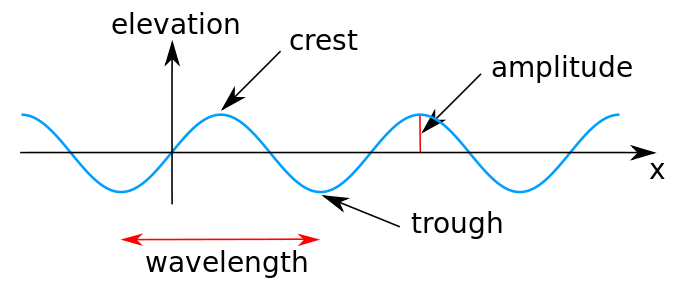
\includegraphics[width=\linewidth]{figs/wave.png}\\
  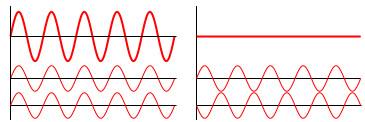
\includegraphics[width=\linewidth]{figs/interference.png}
  \caption{{\it Top}: A simple wave. Local maxima are referred to as {\it
crests}\index{crest} while local minima are {\it troughs}\index{trough}. The
distance between crests is the {\it wavelength}\index{wavelength}. The crest
height is the {\it amplitude}\index{amplitude}. Image taken from
Wikipedia~\cite{wiki:wave}.
{\it Bottom}: Constructive (left) and destructive (right) interference. 
The top wave is created by adding together the bottom two. For example let us
say that the amplitude of the bottom waves is 1 in some units. In the
constructive case, two crests appear at the same point, and so the crest of the
resultant wave will be $1+1=2$. In the destructive case, a crest and trough
appear at the same point and cancel. Image taken from
Wikipedia~\cite{wiki:interfere}.
}
  \label{fig:wave}
\end{figure}

\section{Aspects of quantum physics}\label{sec:QM}

One of the first physical phenomena to reveal to us the extraordinary nature of
short-distance physics was light. Light had been studied for centuries, with
important advances in its understanding coming from the likes of Euclid, Alhazen,
Young, Newton, and Huygens. Through Young and Huygens, light was understood to 
be a {\it wave}\index{wave}, which we will think of in these notes as some function on
space-time that is periodic in space or time or both. A sketch of a simple wave,
along with some related vocabulary is shown in \figref{fig:wave} (top).

Waves represent some kind of departure from an equilibrium state; put another
way, a real wave of one variable with no change from equilibrium would be just 
a straight horizontal line. Departures from equilibrium cost energy, so
intuitively, you can imagine that the more wiggly a wave is, the more energy it
has. A more wiggly wave has a shorter wavelength, so we can intuitively expect
an inverse correlation between the energy of a wave and its wavelength.
When two waves are superimposed on each other, they {\it
interfere}\index{interference}. If the waves mostly work together, they interfere {\it
constructively}, whereas if they mostly cancel each other out, they interfere
{\it destructively}. Examples of totally constructive and totally destructive
interference of a simple way if shown in \figref{fig:wave} (bottom).

To learn that light is a wave, Young performed a {\it double-slit
experiment}\index{double-slit experiment}. The idea is that one shines light
through two small slits in a wall, which then strikes some screen behind the
wall. If light were not a wave, one would expect to see two lit spots on the
screen, directly behind the slits. Instead, what Young found was an interference
pattern like shown in \figref{fig:twoSlit} (top). This {\it interference
pattern}\index{interference!pattern} if light is a wave. A rough explanation of
how that works is depicted in \figref{fig:twoSlit} (bottom).

\begin{figure}
  \centering
  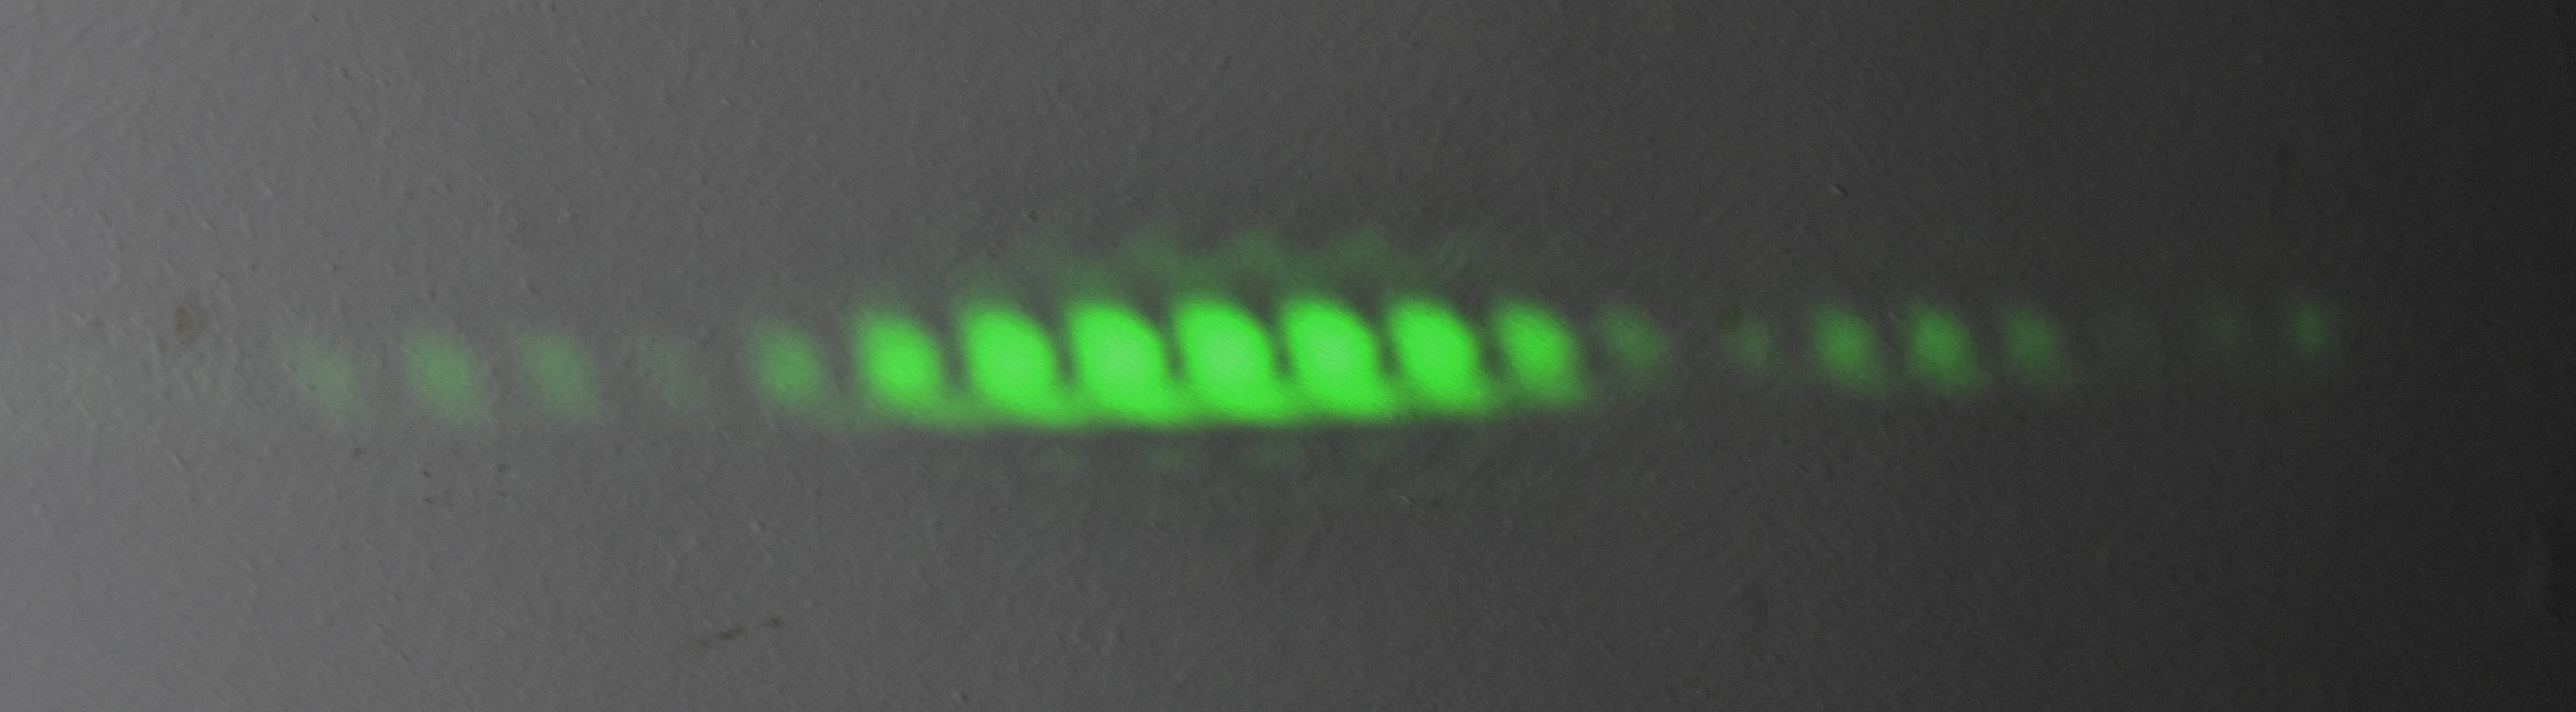
\includegraphics[width=\linewidth]{figs/Youngs_slits.jpg}\\
  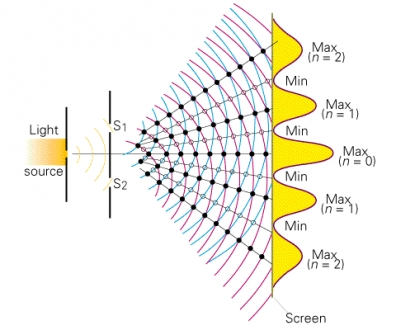
\includegraphics[width=\linewidth]{figs/twoSlitMechanism.jpg}
  \caption{{\it Top}: An example interference pattern one sees when shining green light
through two nearby slits. Image taken from Wikipedia~\cite{wiki:slit}.
{\it Bottom}: Diagram showing the mechanism behind interference patterns. S$_1$
and S$_2$ indicate the slits. The blue and red circle segments indicate maxima
of the waves coming from S$_1$ and S$_2$, respectively. Places where the circle
segments intersect yield complete constructive interference; when these segments are
instead evenly separated, a crest coincides with a trough, giving
complete destructive interference. Image taken from Ref~\cite{deutsch:slit}.}
  \label{fig:twoSlit}
\end{figure}

In the early 1900s, physicists were beginning to see the particle nature of
light. In particular, Planck proposed~\cite{Planck:1901tja}
that light may deliver {\it discrete packets} of
energy, rather than delivering a continuous spectrum of energy\footnote{He was
inspired to propose this because it avoided the\index{ultraviolet catastrophe}
{\it ultraviolet catastrophe}, which is the fact that light with a continuous
energy spectrum and arbitrarily
small wavelength has arbitrarily high intensity, i.e. its intensity diverges.}.
Under Planck's suggestion, light should only be able to have integer multiples
of some set amount of energy, with no other energies possible. Another way we
physicists say this is that the energy must be {\it quantized}. Planck wasn't
sure how this quantization occurred, suggesting for example that perhaps the
walls of a material absorbing light can only absorb quantized energy packets,
for some reason.

Einstein took Planck's idea seriously~\cite{Einstein:1905cc}
and used it to explain the {\it photoelectric
effect}\footnote{This is actually what won Einstein the Nobel, not special or
general relativity. Also in 1905 he published his first
papers on special relativity, as well as a paper on Brownian motion.},
which is the observation that shining light on a material frees electrons. 
In fact, Einstein proposed that this quantization was due to light itself, 
suggesting that light comes
in discrete energy packets. These are the {\it photons}\index{photon}.
A careful study~\cite{millikan_direct_1916} of the photoelectric effect by
Millikan showed that
Einstein's interpretation explained the photoelectric effect well. Finally
Compton showed that light scattered from a particle shifts by the Compton
wavelength\index{wavelength!Compton}
\begin{equation}\label{eq:compton}
  \lambda_c=\frac{\hbar}{2mc},
\end{equation}
where $m$ is the target particle's mass, and $\hbar$ is a constant called
{\it the reduced Planck constant}\index{Planck constant}, 
which one can derive by assuming light
is made of particles with zero rest mass~\cite{Compton:1923zz}.
Altogether these discoveries convinced physicists light behaves as a particle
at short enough length scales. 

As hinted by \equatref{eq:compton}, something else interesting became apparent
around this time: Particles such as electrons also behave like waves. For
example one can carry out the double-slit experiment with electrons, which are
also seen to exhibit interference patterns. Equation~\eqref{eq:compton} assigns
a characteristic wavelength to every particle. Repeating once again the logic of
previous sections, that $\hbar$ and $c$ are constants of nature suggest that
wavelengths and inverse masses can be thought of as ``the same".
This observation that light and matter particles such as electrons can behave as
particles or waves depending on the energy led us to believe that all particles
behave also as wave, a concept called {\it wave-particle
duality}\index{wave-particle duality}. This duality, along with the existence of
discrete energy levels, are two properties of quantum mechanics.


\begin{figure}
  \centering
  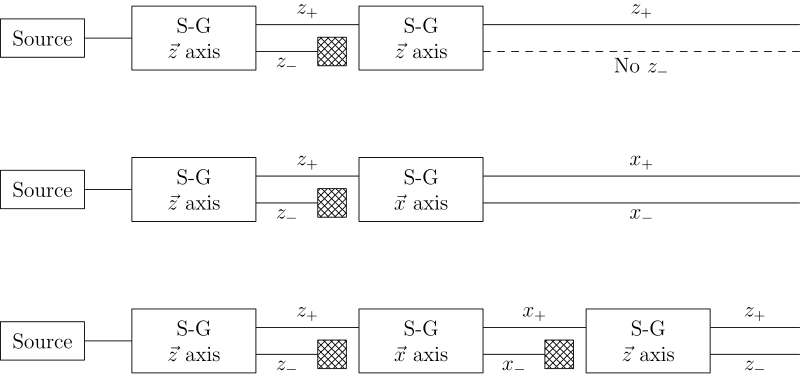
\includegraphics[width=\linewidth]{figs/stern-gerlach.png}
  \caption{Schematic representation of the Stern-Gerlach experiment.
           {\it Top}: A particle has its spin measured along the $\hat{z}$-axis,
which is found to be $+1$. Subsequent measurements along the $\hat{z}$-axis 
will always find +1. {\it Middle}: A particle has its spin measured along the
$\hat{z}$-axis, followed by the $\hat{x}$ axis. The $\hat{x}$-axis spin is
either +1 or -1 with probability 0.5 in each case. {\it Bottom}: A particle has
its $\hat{z}$-axis spin measured, which is found to be +1. A measurement along
the $\hat{x}$-axis destroys our knowledge of its spin, and the following
measurement along the $\hat{z}$-axis is again either +1 or -1 with probability
0.5 in each case. Image taken from Wikipedia~\cite{wiki:SG}. }
  \label{fig:sternGerlach}
\end{figure}

One of the earliest, most important experiments for quantum systems 
was the celebrated Stern-Gerlach
experiment~\cite{gerlach_experimentelle_1922a,gerlach_magnetische_1922b,gerlach_experimentelle_1922c}.
In this experiment, silver atoms were deflected by a magnetic field, which was
used to measure the {\it spin}\index{spin} of the atoms. In general, a
particle's spin is somewhat like its angular momentum\footnote{This statement
comes from the fact that the mathematics for angular momentum and spin are the
same in quantum physics. Physically we understand magnets as follows: Their
magnetic fields are due to the contributions of the spins of all the particles
in the magnet.}, hence the name. A particle's spin influences how it 
interacts with electromagnetic fields. A rough schematic of the Stern-Gerlach
experiment is given in \figref{fig:sternGerlach}.

As suggested in the caption of \figref{fig:sternGerlach}. The Stern-Gerlach
experiment suggests a fundamental randomness to particles. In paricular if you
have a particle, you can't generally predict\footnote{You may wonder if this
randomness is a ``true" randomness, or whether it stands in for some missing
information. For instance if you toss a coin, if you know the exact shape of the
coin, its weight, air resistance, the exact starting position of your hand,
the exact power and path of your throw, and so on, then in principle you can predict how 
the coin will land. It is natural to guess that quantum physics is the same,
that there is some as-yet-underdiscovered hidden information that would allow us
to predict the outcome of a quantum experiment, if only we knew it. If you did
guess this, you'd be in good company, since this 
is what Einstein thought. This hidden information is usually called a {\it
hidden variable}\index{hidden variable} in this context. In the 1960s, Bell
argued on rather general grounds that quantum physics without a hidden variable
must satisfy a certain inequality, which we now call {\it Bell's
inequality}\index{Bell's inequality}~\cite{bell_einstein_1964}. 
Fascinatingly in the early 1980s, Aspect, Grangier, and Roger confirmed Bell's inequality
experimentally~\cite{aspect_experimental_1982}, which is why they got the 2022
Nobel prize. The most likely scenario
therefore appears to be that there is no hidden variable, which means that fundamental
reality is in this sense truly random. Indeed quantum systems are the only
truly random things we are aware of. Other things that appear random, such as
random number generators, are actually deterministic at their foundation.
For completeness, I would like to mention that there are technically ways around 
Bell's inequality. Some of these ways have already been experimentally ruled
out. One possibility that has not yet been ruled out, but which also appears to
not be nearly developed enough to provide experimental predictions, is {\it
superdeterminism}\index{superdeterminism}. A superderministic theory would
underlie quantum mechanics, and my understanding of superdeterminism is that all
experimental outcomes in all space-time should at least in principle be tracable
back to one single set of initial conditions.} 
its $\hat{z}$-component of spin,
unless it has been specially prepared\footnote{In the context of the
Stern-Gerlach experiment, ``specially prepared" means you just took a
measurement along the $\hat{z}$-axis, like in the top row of
\figref{fig:sternGerlach}. That second measurement in the top row 
along the $\hat{z}$-axis is guaranteed to be the same.}. The
Stern-Gerlach experiment reflects a fundamental randomness of the quantum world.
Indeed, for an unprepared system, we can never know an experimental outcome with
absolute certainty. Instead we are limited to expectation values, like those
introduced in \secref{sec:probAndError}. In the Stern-Gerlach experiment, we
know that when measuring an unprepared system, $\ev{\text{$\hat{z}$-spin}}=0$.


\section{Aspects of thermodynamics}\label{sec:thermo}\index{thermodynamics}

{\it Thermodynamics} is effectively the study of very, very large numbers of
microscopic things. A system in thermodynamics is made of some large number of
particles, for instance a gas, and we try to make some statements about the
macroscopic system. For instance you may have learned the {\it ideal gas law} in
a chemistry class. An ideal gas\index{ideal gas} has no interactions, so it
never changes phases. The ideal gas law relates the pressure $P$, volume $V$,
temperature $T$, and number of particles $N$ in an ideal gas as
\begin{equation}
PV=Nk_BT,
\end{equation}
where $k_B$ is a constant of nature called {\it Boltzmann's
constant}\index{Boltzmann constant}. For an monatomic ideal gas, i.e. a gas made
of single atoms as opposed to molecules, the {\it equipartition theorem} relates
the energy contributed by a single particle:
\begin{equation}\label{eq:equipartition}
E_{\text{atom}}=\frac{3}{2}k_BT.
\end{equation}
For the full gas, the energy is thus
\begin{equation}
E_{\text{gas}}=\frac{3}{2}Nk_BT.
\end{equation}
Intuitively one can imagine that increasing the temperature makes the particles
move faster, leading to more collisions. Correspondingly at fixed volume, the
pressure would increase, in agreement with the ideal gas law.
The equipartition theorem is one example that suggests that energy and
temperature for the ideal gas are the same up to a constant.


\section{The natural unit system}\label{sec:units}

The units that you have seen, the [kg], the [m], and so on, belong to the {\it
SI unit system}\index{units!SI}. Still, in the preceding sections, 
we have had a repeating perspective that two
quantities with fundamentally different units are related by some constant of
nature, either $c$, $\hbar$, or $k_B$, and may therefore be thought of as 
more or less ``the same".
The {\it natural unit} system takes this ideal to the extreme.

Natural units are a convenient way to do manipulations without having to keep
track of all the fundamental constants as they enter a calculation. One forgets 
about these constants (sets them equal to one) then restores
them at the end of a calculation. For example let us eliminate the speed of light
by setting $c=1$. Then \equatref{eq:emc2} becomes
\begin{equation}\label{eq:massEnergyNatural}
E=m.
\end{equation}
If I square the above equation I find
\begin{equation}
E^2=m^2.
\end{equation}
Now let's say I want to switch back to SI units. I can accomplish this through
dimensional analysis by figuring out how many powers of $c$ I have to put on
the RHS to get the SI units to make sense. In this extremely trivial example,
one does not gain much from natural units. For much more intensive calculations,
it becomes extremely tedious and error-prone to carry the powers of $c$ at each
step, while providing no useful information, and therefore natural units are
extremely useful in such situations.

The full prescription\footnote{One may also set Newton's gravitational constant
$G=1$ when gravity is relevant to the calculation.} of natural units is to set
\begin{equation}
\hbar=c=k_B=1.
\end{equation}
Through natural units, every physical quantity has only one fundamental unit,
which can be expressed either as some power of
energy or equivalently some power of inverse length. As discussed in
\secref{sec:EM}, the favorite unit of energy for particle physics is the [eV].
Hence it is typical to see particle masses expressed in [eV]. In these units,
the proton mass is
\begin{equation}\label{eq:massp}
m_p=938\units{MeV}.
\end{equation}
Meanwhile the temperature of the center of the sun, which in SI units is about
15 million Kelvin, comes out to a measly
\begin{equation}\label{eq:Tsun}
T_{\text{center}}=1.2\units{keV}.
\end{equation}
When we particle physicists are interested in lengths, we like to use
the femtometer [fm], which is $10^{-15}$ [m]. Owing to the fact $c=1$, speed is
unitless in this system.


\section{The Standard Model}\label{sec:SM}

The Standard Model (SM) of particle physics classifies all 
known\index{particle!elementary}\index{Standard Model}
{\it elementary particles}, i.e. particles with no known substructure,
and describes three fundamental forces:\index{force!fundamental} the EM,
{\it weak}\index{force!weak}, and {\it strong}\index{force!strong} forces. 
You are likely already familiar with the EM force, which is the
phenomenon we harness for lights, televisions, radios, microwaves, and so on.
The weak force allows for certain nuclear decay processes to occur; that's all
we'll say about it for now. The strong force holds together protons and neutrons
inside of atoms\footnote{If you think about it, such a force must exist. After
all, protons have positive electric charge, and neutrons have no electric
charge. If there were no strong force, atomic nuclei would just fly apart, since
like charges repel.}. The only remaining fundamental force that has not yet been
brought into the fold is gravity\footnote{Attempts to describe gravity using the
same kind of framework as the SM are sometimes called {\it quantum gravity},
which you may have heard of before. Theories of quantum gravity are troubled by
a technical problem: they are {\it non-renormalizable}. This means the theory is
plagued with infinities that cannot be removed in a systematic way, at least not
like they can be removed in the SM.}, which we understand through a separate
framework called\index{relativity!general} {\it general relativity}.

Elementary particles can be divided into
\index{particle!matter}
{\it matter particles} (quarks and leptons); gauge bosons, which
I mentioned in \secref{sec:groupsMatter} and which mediate
\index{boson!scalar}\index{boson!gauge}
the three aforementioned forces\footnote{Again, not gravity.}; 
and a\index{boson!scalar} {\it scalar boson}, the Higgs boson,
whose field interacts directly with some elementary particles that thereby
acquire their mass. For each particle there exists a corresponding
{\it antiparticle}\index{antiparticle}. Antiparticles have the same mass as
their partner particle, but they have opposite charges. For example the
antiparticle for an up quark, which has electric charge +2/3, that furthermore
has red color charge, is the anti-up, which has electric charge -2/3 and antired
color charge. Antiparticles are indicated with a bar, so a generic antiquark is
written $\bar{q}$.

\begin{figure}
  \centering
  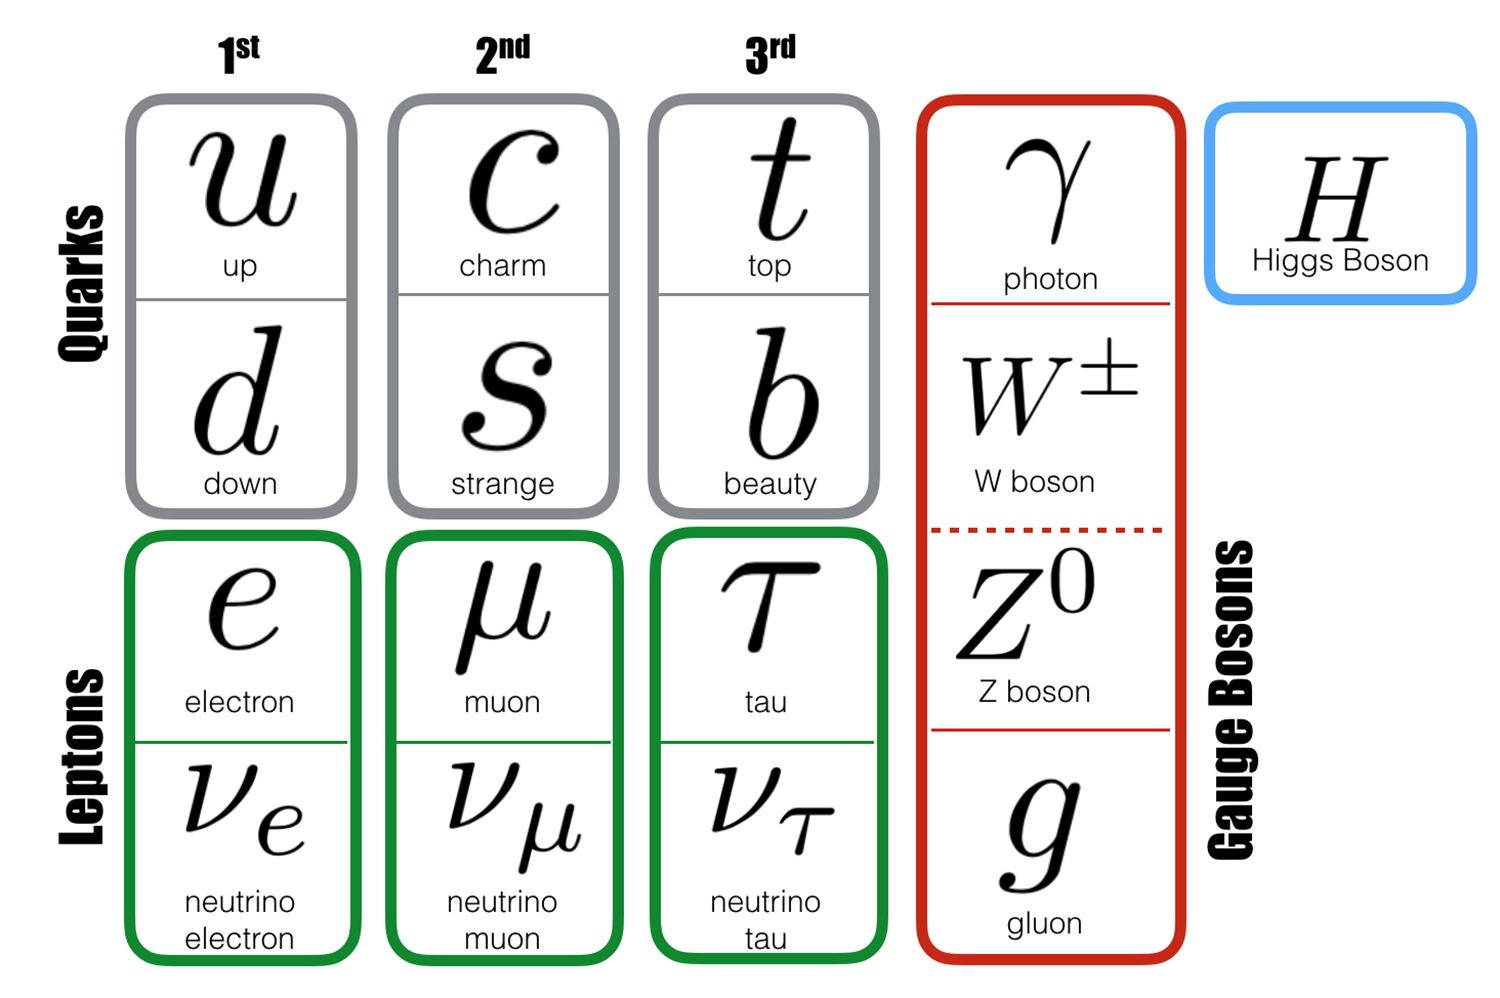
\includegraphics[width=\linewidth]{figs/SM.png}
  \caption{Summary of elementary SM particles. The first three columns give
           the three generations of matter particles. Image taken
           from the Physics Institute at University of
           Zurich~\cite{zurich_SM}.}
  \label{fig:SM}
\end{figure}

Figure~\ref{fig:SM} gives a schematic overview of the SM.
In the first three columns are all the known matter particles.
Matter particles can be divided into\index{quark} {\it quarks}
and\index{lepton} {\it leptons}. Quarks make up so-called {\it hadrons},
the most familiar of which to you would be protons and neutrons; for
example a proton is made of two up quarks and a down quark. Quarks can feel the
strong force, the EM force, the weak force, and the Higgs. 
Leptons differ from quarks in that they do not feel the strong force; moreover
we do not believe the neutrinos feel\footnote{Nevertheless, they appear to be
massive. How neutrinos acquire their masses is an area of active research in
particle physics.} the Higgs. The electron is the lepton most
familiar to you. Quarks and leptons can be divided into three\index{generation}
{\it generations}, which are indicated at the top of each column.
Masses distinguish\footnote{The later generations are heavier than the earlier
generations. This is not true for neutrinos, whose mass ordering has yet to be
determined.} the various generations; for instance the top quark is
heavier than the charm, which is heavier than the up, even though they all have
electric charge $+2/3$.

The fourth column we find the gauge bosons, which\index{mediate} 
{\it mediate} the fundamental forces, i.e. we believe that particles feel forces
by exchanging gauge bosons. For example, the photon mediates the EM interaction.
When two electrons repel from each other, from the modern perspective of
particle physics, this occurs because they are exchanging photons.
As discussed in \secref{sec:groupsMatter}, gauge bosons are a physical
manifestation of underlying symmetries. The photon and $W$ and $Z$ bosons
are manifestations of a combined $\SU(2)\times\U(1)$ symmetry. Meanwhile the
gluon is a manifestation of an $\SU(3)$ gauge symmetry.

Sometimes it is useful to focus on only part of the SM. In the case of lattice
calculations, one reason to do this is that the more particles you add to a
simulation, the more expensive it becomes. The strong force is also special
because it has a well-defined {\it continuum limit}, which we will discuss in
\chref{ch:LFT}. For these reasons, lattice simulations focus on systems with
only quarks and gluons. This is the realm of QCD, and lattice simulations of QCD
are usually called lattice QCD (LQCD). 

\subsection{Fields}\label{sec:fields}

As already mentioned in \secref{sec:SR}, a field is some math object defined on
all space and time, and I gave the simple example of temperature as a scalar
field. From the perspective of modern physics, all particles are understood as
manifestations of underlying fields. Hence there is a photon field, and electron
field, and so on. Fields whose manifestations are quarks and leptons are called
{\it matter fields}\index{field!matter}. Similarly, fields whose manifestations
are gauge bosons are {\it gauge fields}\index{field!gauge}.

\begin{figure}
  \centering
  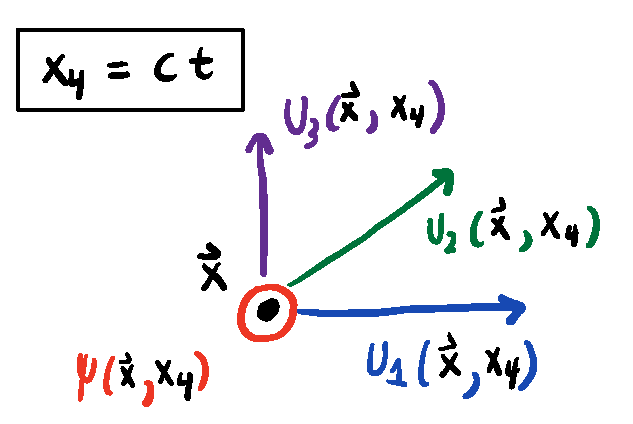
\includegraphics[width=0.6\linewidth]{figs/fields.pdf}
  \caption{A schematic drawing of some fields associated with a space-time point
           $\fvec{x}=(\vec{x},x_4)$. In this theory there is a matter field
           $\psi(\fvec{x})$ and a gauge field $U_\mu(\fvec{x})$ with four
           components labeled by $\mu$, $1\leq\mu\leq4$.
           We can only show three spatial components (directions) of the gauge field 
           $U_1(\fvec{x})$, $U_2(\fvec{x})$, and $U_3(\fvec{x})$.}
  \label{fig:fields}
\end{figure}

Fields play an extremely important role in the formalism of the SM, which is
usually called {\it quantum field theory} QFT. Introducing matter fields with a
particular mathematical structure allows them to be compatible with special
relativity; in fact the whole QFT formalism was born out of an attempt to make
quantum mechanics compatible with special relativity. They also are important in
another way: they proffer an explanation why particles are exactly identical.
Indeed the fact that all photons are indistinguishable, all electrons are
indistinguishable, and so on, is a conclusion one reaches when learning
statistical physics.
Matter fields are introduced as a math object called a {\it spinor}, which can
be expressed as a complex vector. Gauge fields, meanwhile, can be expressed as
matrices ``that point in a direction", i.e. in a 4-$d$ space-time, there are
four gauge fields associated to each space-time point. A schematic
representation of this is given in \figref{fig:fields}.

Let us gain a bit more geometric intuition for these gauge matrices. We will
start with the gauge group $\U(1)$ and work our way up in complexity.
Recall from \secref{sec:groupsMatter} that $\U(1)$ could be identified with the
set of rotations of a circle. Hence, for a theory that has an underlying gauge
group $\U(1)$, you can imagine at each point in space and time something
like \figref{fig:fields}, where each colored arrow could be any point on a
circle\footnote{The arrows in the figure are just supposed to emphasize that
there are four matrices per space-time point, one associated with each direction
$x$, $y$, $z$, and $t$. In the case of $\U(1)$, you can at least schematically
think of each gauge matrix as a circle attached to each arrow. Generically
speaking, varying the gauge field is equivalent to spinning all the circles
attached to all the arrows of every space-time point.}.

The next-most interesting gauge group is $\SU(2)$. It can be represented as
\begin{equation}
\SU(2)=\left\{
\left(\begin{array}{cc}
          a+ib   & -c+id  \\
          c+id   &  a-ib  \\
            \end{array}\right)\suchthat a,b,c,d\in\R \right\}.
\end{equation} 
One property of $\SU(N)$ matrices, $N\in\N$, is that they have determinant 1.
This leads to the constraint
\begin{equation}
a^2+b^2+c^2+d^2=1,
\end{equation}
which is the equation for the unit hypersphere in four dimensions, often 
denoted\footnote{In general, $S^m$ is the unit hypersphere in $m+1$ dimensions.}
$S^3$. We can therefore think of $\SU(2)$ elements as points on $S^3$.

The group that is actually relevant for strong interactions is $\SU(3)$. Because
of the above two situations, I always sort of figured that $\SU(3)$ could be
thought of as a point on $S^8$. Unfortunately this is not the case. Still,
$\SU(3)$ elements are characterized completely by eight angles, in such a way
that you can sort of imagine it as two hyperspherical surfaces $S^5$ and $S^3$
somehow\footnote{I guess the correct statement is something like ``$\SU(3)$
is the total space of an $S^3$ fibration over $S^5$." I don't really know what
that means, hence the entangled hyperspheres metaphor. I guess if you eventually
choose to take differential geometry, you will learn.} entangled with each other.


%The theoretical framework underlying the SM is an example of a Quantum
%Field Theory (QFT). QFTs are consistent with both quantum mechanics and
%relativity. Lattice gauge theories are a kind of QFT; therefore it is
%important for the reader to know a little bit about them. There are a lot
%of different resources one can use to learn about QFT; for example when I was a
%grad student I used Peskin and Schroeder~\cite{peskin_introduction_1995}
%and Srednicki~\cite{srednicki_quantum_2007}.
%Nowadays there are also some very high quality lectures on YouTube,
%for instance a series by Tong~\cite{tongQFT}, which I found had some other nice
%introductory remarks.
%A timeline of particle discoveries can be found in
%Ref.~\cite{wiki_particle_discoveries}. Another detailed historical overview
%of the SM is given in Chapter 1 of Ref.~\cite{griffiths_introduction_2007}.

\section{Further reading}

At some point in your career, you should learn each of these subjects in some
careful detail. Here I collect some resources that I found helpful when I was an
undergraduate. 
\begin{itemize}
  \item Electrodynamics: For this subject, the standard favorite is
Griffiths's {\it Introduction to electrodynamics}~\cite{Griffiths:1492149}.
You will see that Griffiths makes a lot of nice physics books at the
undergraduate level.
  \item Special and general relativity:
A good starting point is Moore's {\it Six Ideas that Shaped Physics: Unit
R}~\cite{moore2002six}. A nice next step would be {\it Relativity, Gravitation,
and Cosmology: A Basic Introduction} by Cheng~\cite{alma997111578601771}.
  \item Quantum mechanics:
Most classes use Griffiths's {\it Introduction of Quantum
Mechanics}~\cite{griffiths_introduction_2005}. This is a nice book, and I especially enjoy
its discussion at the end of Bell's inequality\footnote{Which you may want to
read at some point, seeing as the 2022 Nobel prize in physics was the
experimental verification of this.}. Still my favorite is Shankar's
{\it Principles of Quantum Mechanics}~\cite{Shankar:102017}, which contains an
extremely helpful mathematical introduction.
  \item Thermodynamics:
Shroeder's {\it An Introduction to Thermal
Physics}~\cite{schroeder2021introduction} is the only book at the undergraduate
level I have tried.
  \item Particle physics:
{\it Introduction to Elementary Particles} by
Griffiths~\cite{griffiths_introduction_2007} explains some of the basic ideas of
modern particle physics and has a nice history in the beginning. Thomson's
{\it Modern Particle Physics}~\cite{thomson_modern_2013} is certainly accessible to an advanced
undergraduate and more up-to-date, including for instance an elementary
explanation of the Higgs mechanism.
\end{itemize}

\section*{Exercises}

For Exercises (1-5), write a Python function that:
\begin{enumerate}
    \item converts between [mi] and [m];
    \item converts between [s], [min], [h], and [y];
    \item converts between [lb] and [kg], assuming you’re close to the earth’s surface;
    \item given an object with some mass and height above the earth’s surface, can 
          calculate how much gravitational potential energy in [J] the object has; and
    \item converts between [m] and [ly].
    \item A tank weighs about 140,000 [lbs]. Use your program from problem (4) 
          to calculate how much gravitational potential energy in [J] the tank has when 
          it’s 1 [mi] off the ground.
    \item Assuming an apple has a mass of 100 [g], calculate its rest mass energy.
    \item Suppose you could magically convert 100\% of an apple’s rest mass into energy, 
          and then use that energy to lift a tank off the ground. How far off the 
          ground could you lift it?
    \item Write a python script that converts between [MeV] and [fm$^{-1}$].
          Also write a script that converts between [fm] and [MeV$^{-1}$].
    \item Working in the natural unit system, express the units of power, pressure,
          and momentum as a power of [MeV]. Repeat for [fm].
    \item What is your height in [MeV$^{-1}$]?
    \item Use \equatref{eq:massp} to determine the proton mass in [kg].
    \item Show that \equatref{eq:Tsun} is correct.
\end{enumerate}

\bibliographystyle{unsrtnat}
\bibliography{bibliography}

\chapter{A sketch of lattice field theory}\label{ch:LFT}

LFT was first dreamt up by Kenneth Wilson\footnote{Wilson was more of a condensed
matter theorist at that time. Back then, people were still working out the SM,
fueled by a cavalcade of rapid experimental discoveries of new particles. For
Wilson, particle physics seemed very exciting, and he wanted in on the action.
Since his expertise was not in high energy theory, he took an approach more
informed by condensed matter, which led to his lattice formulation. Indeed, his
approach makes plain many powerful, formal correspondences between lattice field
theories and {\it spin models}\index{spin model}, which are models that explain
how magnets work by imagining them as a solid block of interacting spins.} 
in 1974~\cite{wilson_confinement_1974}.
He used this formalism to explain a phenomenon called {\it quark
confinement}\index{quark confinement}, which is the observation that one never
finds a quark alone in nature. He considered an infinitely heavy quark-antiquark
pair and calculated its potential energy in the lattice formalism. He found
\begin{equation}
V_{\bar{q}q}(r)\sim\frac{A}{r}+\sigma r,
\end{equation}
where $r$ is the separation between the quarks and $\sigma$ is a positive 
constant called the {\it string tension}\index{string tension}. The first term 
is reminiscent of the Coulomb potential energy from electrodynamics, so it is 
often called the ``Coulomb part". In contrast with the EM Coulomb interaction, 
this part of the potential, is repulsive between the quark-antiquark pair.
When $r$ is small, this term dominates. When $r$ is large, the second term
dominates, and the potential increases with $r$.
How this leads to confinement is sketched pictorially
in \figref{fig:confinement}. 

\begin{figure}
  \centering
  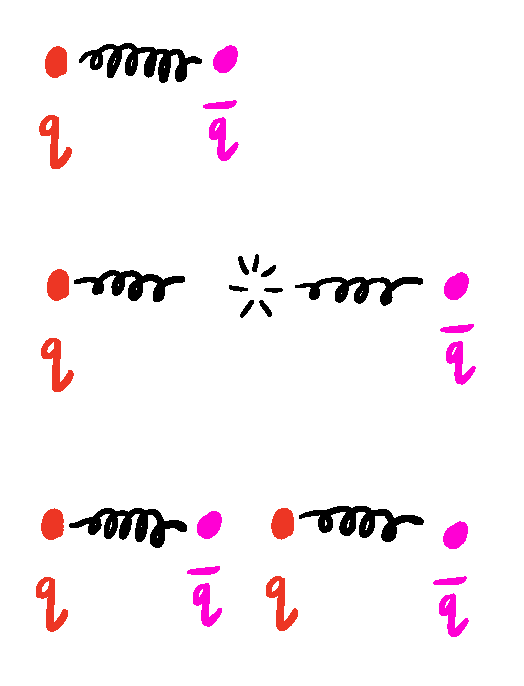
\includegraphics[width=0.8\linewidth]{figs/confinement.pdf}
  \caption{A sketch of the confinement phenomenon. {\it Top}: A quark-antiquark
pair bound together through the strong interaction. {\it Middle}: The quark and
antiquark are separated, which increases the potential energy between the
quarks. Eventually this energy becomes so high, the binding ``breaks".
{\it Bottom}: The binding breaks because the potential energy exceeds the rest
mass energy of another quark-antiquark pair. Therefore it is energetically
favorable to generate such a pair from the vacuum, which is what is shown here.
Thus from one quark-antiquark pair there spawns two.} 
  \label{fig:confinement} 
\end{figure}

At first, people thought that lattice simulations would not be computationally
viable, Wilson included. This attitude changed in 1979 when Michael Creutz, 
working at Brookhaven
National Lab, carried out the first lattice study, at that time using the gauge
group\footnote{You can think of this group like a simplified version of
$\SU(3)$, which again is the gauge group corresponding to real-world gluons.
$\SU(2)$ has a lot of qualitative similarities to $\SU(3)$, while being
computationally much, much cheaper. Therefore lattice practitioners sometimes
like to use $\SU(2)$ as a testing ground. In fact when I was a grad student, the
systems I studied only had $\SU(2)$ ``gluons".} $\SU(2)$~\cite{creutz_monte_1980}. 
Creutz's success excited the high
energy community very much. Early computers were far too weak to simulate realistic
quarks, so studies were limited to theories with gluons only. Over the last
decades, advancements in computer hardware and computing algorithms, along with 
better theoretical control over implementations of lattice field theories on
computers, have allowed us to simulate most of the QCD sector. State-of-the-art 
calculations include, in addition to gluons, physically realistic up, down,
strange, and charm quarks.

I now attempt to give a sketch of how LFT works. In nature we
exist in a 4-$d$ space-time; correspondingly LFT will have a 4-$d$ domain. The
trick with LFT is to imagine that the space-time is {\it
discrete}\index{discrete}; i.e. that there is a minimum distance between points.
One usually looks at a small region of space-time, represented by a 4-$d$
box\footnote{In higher dimensions, one sometimes calls rectangles
{\it orthotopes}\index{orthotope}.}. Setting up this discrete lattice renders
the previously uncountably infinite domain finite and countable. Since the
theory can now be specified by finitely many numbers, we are able to store it in
a computer's memory.

At this stage I would like to emphasize that {\it the lattice is in no way
real}. It is a calculational crutch that allows us to utilize methods of scientific
computing\footnote{There are other technical advantages as well, but getting
into them is far beyond the scope of these notes.}. As we increase the finite
number of discrete points on our lattice while simultaneously decreasing the
lattice spacing, we obtain an increasingly accurate depiction of reality in that
space-time box. By extrapolating to the limit of zero lattice spacing, we hope
to lose all reference to the lattice; put another way, our crutch disappears.

In the following sections, I will try to explain these ideas in a little more
detail. I don't expect you to understand things fully, because I am not
explaining them fully. It is enough for you to have a heuristic understanding of
what a lattice calculation entails. 


\section{Defining the lattice}

Let $N_{1},N_{2},N_{3},N_{4}\in \N\cup\{0\}$. The {\it lattice} ${\Lambda}$ is defined by
\begin{equation}
  {\Lambda}\equiv\{\fvec{x}\suchthat x_\mu=a\,n_\mu,\,n_\mu< N_\mu,\,
      \mu=1,2,3,4\}.
\end{equation}
Here $a$ is called the \index{lattice spacing}{\it lattice spacing}.
The subscript $\mu$ indicates the $\mu$-component of the four vector $\fvec{x}$.
We identify $N_1$, $N_2$, and $N_3$
as the extensions of the lattice in the spatial directions,
and $N_4$ is taken to be the extension in the time
direction. Matter fields 
are defined on the \index{site} {\it sites} $\fvec{x}\in\Lambda$. We shall
take the lattice to have periodic\footnote{Real life does not have periodic BCs.
We like to implement periodic BCs on the lattice in part because they allow for
symmetries under translations. You may protest that because real life doesn't
have periodic BCs, it is not reasonable to implement them on the lattice. One
reason this can be justified is as follows: Physical quantities that are small
compared to the box size tend not to ``feel" the BCs very strongly. This
manifests in principle as a systematic error that decreases, often
exponentially, with increasing box size. As long as the box is large enough, 
this systematic error is swallowed by
the statistical error, i.e. it is negligible.} boundary conditions (BCs), i.e.
\begin{equation}\label{eq:PBC}
  \fvec{x}+aN_{\mu}\hat{\mu}=\fvec{x},
\end{equation}
where $\hat{\mu}$ is the unit vector\footnote{Hence $a\hat{\mu}$ marches one 
step in the $\muh$-direction.} in the direction indicated by $\mu$.
An example of this setup in two dimensions is given in \figref{fig:lattice}.

\begin{figure}
  \centering
  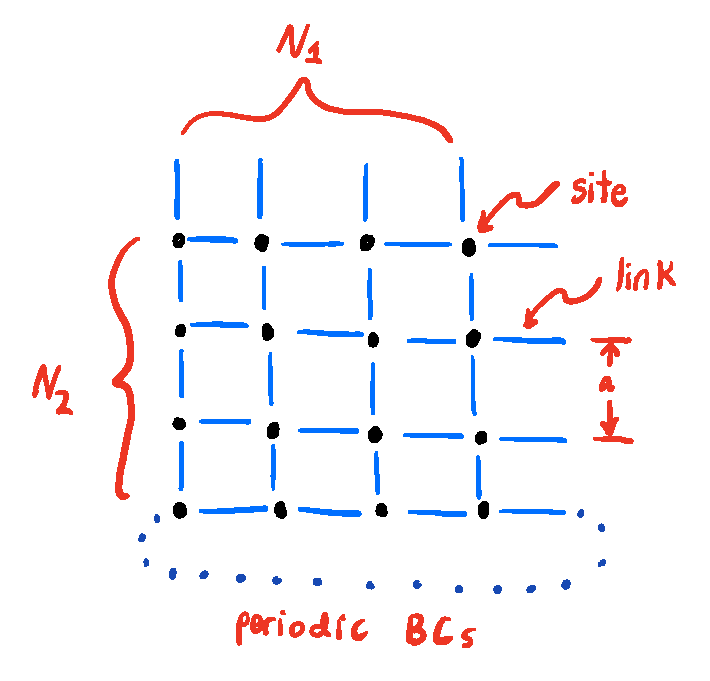
\includegraphics[width=\linewidth]{figs/lattice2d.pdf}
  \caption{A 2-$d$ lattice with $N_1=N_2=4$. Sites are indicated by black dots
and links are indicated by blue lines. Matter fields live on the sites and gauge
fields live on the links connecting the sites. The dotted, dark blue line 
indicates periodic BCs,
i.e. if I start at the bottom-right site and march one step to the right
($\mu=1$ direction in this example), I will end up at the bottom-left site.}
  \label{fig:lattice} 
\end{figure}

Let us explore some of the consequences of treating space-time as discrete
and putting it in a box.
There are many, but we will here focus only on a few of the most easy-to-grasp
ones. First of all, derivatives are given by
by finite differences,
\begin{equation}\label{eq:dertodiff}
  \partial_\mu f(\fvec{x})\to\Delta_{\mu}f(\fvec{x})\equiv\frac{f(\fvec{x}+a\hat{\mu})
                                                   -f(\fvec{x}-a\hat{\mu})}{2a}.
\end{equation}
Note that if one takes the limit $a\to0$, one recovers the definition of a derivative.
We similarly replace integrals with sums,
\begin{equation}\label{eq:inttosum}
  \int \dd[4]{\fvec{x}}f(\fvec{x})\to a^4\sum_\fvec{x}f(\fvec{x}).
\end{equation}
In the limit $a\to0$, letting the number of sites grow to infinity, while
keeping the box size fixed, one gets a Riemann sum, i.e. one gets the familiar
integral again. 
This limiting procedure is called the {\it continuum limit}\index{continuum
limit}, and we expect that we recover real-world results in that limit. 
The continuum limit is shown schematically in \figref{fig:climit}.

\begin{figure}
  \centering
  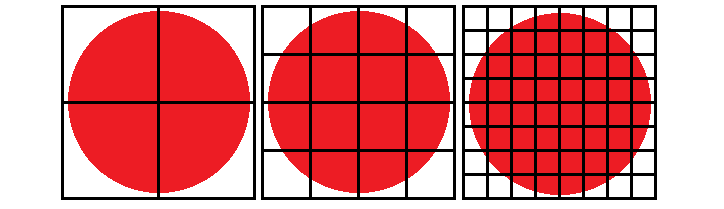
\includegraphics[width=0.9\linewidth]{figs/continuumlimit.png}
  \caption{A schematic representation of the continuum limit. The
           red object represents some physical quantity. As the
           images progress to the right, the lattice spacing decreases
           while the number of sites increases, increasing the resolution.}
  \label{fig:climit}
\end{figure}


There are also some ways physics gets changed when placed on a
discrete lattice in a box, rather than existing in a continuous space-time of
infinite size. In \secref{sec:QM}, we saw that each elementary particle has a
characteristic wavelength. On a finite, discrete lattice, the allowed wavelengths 
of particles are limited.
Heuristically, the lattice does not accommodate particles with a wavelength
smaller than $a$. It also does not accommodate particles whose wavelength is
longer than the box size. This can distort results on a single lattice. The
distortion weakens as one decreases the lattice spacing and increases the box
size, sort of like how a picture gets clearer when one increases the resolution
of a camera. Again, the expectation is that these effects disappear completely
in the continuum limit. 


\section{Constructing measurable quantities}

For the remainder of this chapter, we are going to forget about matter fields.
Again the purpose of these notes is to give the reader an intuitive
understanding of LFT, and introducing fermion fields gives rise to some
technical challenges. Therefore we are going to restrict our attention to a
theory with gauge fields only, i.e. a theory with gluons as the only particles.
Such theories are sometimes called {\it pure gauge} theories\footnote{If the
gauge group is $\SU(3)$ like it is with QCD, we may even call it a pure
$\SU(3)$ theory.}, and we call
pure gauge theories on the lattice {\it lattice gauge theories} (LGT).

Now that we've sacrificed all particles but the gluon, you may worry there is no
physics remaining from which one can learn something. Thankfully it turns out
that a theory with only gluons and a theory with quarks that have infinite mass
are formally equivalent. Thus leaving out quarks that are already heavy to begin
with, such as the charm quark, is often a good approximation. For the lighter
quarks, one generally picks up some non-negligible systematic error that is not 
always easy to predict. 

Next we define the building blocks necessary to construct gluonic observables on the
lattice. The directed {\it link}\index{link}\footnote{In some older texts one
also sometimes sees the phrase ``link variable".\index{link variable}} 
connects $\fvec{x}$ with the
neighboring point $\fvec{x}+a\hat{\mu}$. We indicate it as 
$U_\mu(\fvec{x})\in \SU(3)$. Since we will be interested in $\SU(3)$ for the
remainder of the text, we denote the identity matrix in $\SU(3)$ as $\id$.
A link is
indicated in \figref{fig:lattice}.
We associate to any path $\mathcal{C}$ one can draw on the lattice
the ordered product of its links  $U(\mathcal{C})$.
If we follow a path and then reverse our steps, we should end
up back where we started; hence
\begin{equation}
  U_{-\mu}(\fvec{x}+a\hat{\mu})U_\mu(\fvec{x})=\id.
\end{equation}
Furthermore $U^\dagger(\fvec{x})U(\fvec{x})=\id$, since $\SU(3)$ is a unitary
group, so we can see the effect
of the dagger on links:
\begin{equation}
  U_\mu^\dagger(\fvec{x})=U_{-\mu}(\fvec{x}+a\hat{\mu}).
\end{equation}
Let $\mathcal{C}_{\fvec{x}}$ be a path on the lattice that originates and
terminates at the point $\fvec{x}$. The corresponding {\it Wilson loop} is
defined by \index{Wilson!loop}$\tr U(\mathcal{C}_{\fvec{x}})$.
All of our observables will be Wilson loops of some kind.

The first observable we will look at is the so-called plaquette.
A\index{plaquette}
{\it plaquette} is the
smallest Wilson loop, an oriented square of side length $a$ with
corresponding link product
\begin{equation}
  \plaq_{\mu\nu}(\fvec{x})=U_\mu(\fvec{x})U_\nu(\fvec{x}+a\hat{\mu})
                        U^\dagger_\mu(\fvec{x}+a\hat{\nu})U^\dagger_\nu(\fvec{x}).
\end{equation}
It turns out that the plaquette is related to the gluonic energy density; i.e.
\begin{equation}\label{eq:edensity}
\ev{\tr\plaq_{\mu\nu}(\fvec{x})}\sim \frac{E}{6V_4}\equiv\epsilon,
\end{equation}
where $V_4$ is the number of sites on the 4-$d$ lattice. The factor 6 comes
because every site in 4-$d$ LGT touches six plaquettes\footnote{In $n$
dimensions, each site $\fvec{x}$ has $n!/2(n-2)!$ positively oriented (the links
curve in the CCW direction) plaquettes
with a link starting at $\fvec{x}$ and pointing away from it. This is equal to the
number of unique combinations of directions. Each link has $2(n-1)$ staples
attached to it.}. The lattice representation of a physical observable is called an {\it
interpolator}; hence the plaquette is an interpolator for the energy density.


In \equatref{eq:edensity}, the desired observable we want to learn about the
system is its energy density. In practice, we can estimate the LHS on one
lattice by calculating the average plaquette on that lattice, i.e. we calculate
the plaquette at every site for all six orientations, then take the arithmetic
mean. This gives us a {\it measurement} of the energy density on the $i\nth$
lattice,
\begin{equation}
\epsilon_i=\frac{1}{6V_4}\sum_{\fvec{x},\mu<\nu}\tr\plaq_{\mu\nu}(\fvec{x}).
\end{equation} 
We will discuss how one generates the $i\nth$ lattice in \secref{sec:steps}.



\section{Recovering numbers with units}

Lattice computations deliver quantities
\begin{equation}\label{eq:latticemass}
M=am,
\end{equation} 
where
$m$ is some physical mass. For example $m$ could be the proton mass in [MeV].
The lattice spacing $a$ has units of [MeV$^{-1}$] (equivalently units of
length), which means that $M$ is unitless. We sometimes like to 
think about $a$ being unitless with $a=1$, which we call
{\it lattice units}\index{units!lattice}. This is a useful way to think
when you consider that a lattice is implemented on the computer. For
instance a space-time point on the lattice will be represented as an integer
tuple\footnote{More precisely, space-time will be represented as an array. One
has to find a bijection between space-time points on the lattice and array
indices, which is called {\it indexing}\index{indexing}. The indexer is used all
the time; therefore how one implements an indexer can have a sizable impact on
the performance of the code.} in the computer $(n_1,n_2,n_3,n_4)$, 
which naturally has no units, and it
is furthermore separated by its nearest neighbors by 1.
Moreover, when starting a brand new project, we are often in a situation where
we don't yet know the lattice spacing.

This raises the obvious question of how one determines $a$. One strategy is to
pick a mass that you already know from experiment. The above example of the
proton is well known, i.e. in that case we know $m$. Knowing $m$, one recovers
the lattice spacing as
\begin{equation}
a=\frac{M}{m}.
\end{equation}
Of course, there are many quantities we know experimentally. Depending on the
project, it may be advantageous to use one mass over another. The act of
choosing a mass to use to determine $a$ is called {\it scale
setting}\index{scale setting},  
and commonly one says something like ``we set the scale with the proton mass."
In this example, we call the proton mass the {\it reference
scale}\index{reference scale}.

Once we know $a$, we are able to determine any physical quantity, so long as we
know its interpolator. This is one of the most elegant characteristics of LFT:
It takes only one input parameter, the reference scale, and everything else
with physical units can be calculated from that, using another equation with the
form \eqref{eq:latticemass}.



\section{Computer implementation}

The goal of a lattice program is to estimate the expectation value of some
physical observable $X$, $\ev{X}$, by randomly generating configurations $C$
distributed with probability $e^{-E(C)}\dd C$, where $E(C)$ is the energy of that
configuration. Remember from \secref{sec:QM}, we know that quantum physics tells
us we are limited to knowing expectation values of experimental outcomes rather
than the exact experimental outcome itself.

Extracting this expectation value generally works as follows:
On each configuration $C_i$, we make a measurement $X_i$, which we can think of
as a random variable. The average
\begin{equation}\label{eq:arithmeticaverage}
  \bar{X}=\frac{1}{\nconf}\sum_{i=1}^{\nconf} X_i,
\end{equation}
where $\nconf$ is the number of generated configurations,
serves as the estimator for $\ev{X}$. From the CLT 
we know that, provided we did everything correctly, $\ev{X}$ should
be at most $\sigma_{\bar{X}}$ away from $\bar{X}$ about 68\% of the time.
Provided we did everything correctly, we should have
\begin{equation}
\lim_{\nconf\to\infty}\hat{X}=\ev{X}.
\end{equation}

To generate our configurations, we start from some arbitrary configuration
$C_0$ and construct a stochastic sequence of configurations.
Configuration $C_i$ is generated based on\index{update}
configuration $C_{i-1}$, which we call an {\it update} or {\it Monte Carlo
step}\footnote{The idea of Monte Carlo algorithms dates back to the 1940s.
Stanislav Ulam wanted to know the probability of winning a game of Solitaire.
The calculation turned out to be too complicated to do by hand, so he wanted to
estimate this by playing repeated games, then calculating
$$
{\rm win\ chance}\approx\frac{\rm number\ of\ wins}{\rm number\ of\ games}.
$$
Of course this is tremendously tedious; it is much more appropriate for a
computer. Other scientists working with him at Los Alamos such as John von
Neumann and Nicholas Metropolis are early pioneers of this method.}.
The result is a {\it Markov chain}
\begin{equation}\label{eq:markov}
  C_0\to C_1\to C_2\to...
\end{equation}
of configurations.

Since $C_i$ is generated based on $C_{i-1}$, measurements on subsequent
configurations are correlated. 
One way to reduce these correlations is to separate
configurations are separated by many, many updates.
To check whether the final data are effectively independent, one can use
the {\it integrated autocorrelation time}.
For statistically independent measurements, we expect the variance 
$\sigma^2_{\bar{X}}$ of $\bar{X}$ to be
\begin{equation}
  \sigma^2_{\bar{X}}=\frac{\sigma^2}{\nconf}
\end{equation}
due to the CLT. In practice, however, one finds
\begin{equation}
  \sigma^2_{\bar{X}}=\frac{\sigma^2}{\nconf}\tauint.
\end{equation}
The\index{autocorrelation time!integrated}
factor $\tauint$ is the integrated autocorrelation time. It is the
ratio between the estimated variance of the sample
mean and what this variance would have been if the data were independent.
For effectively independent data, $\tauint=1$.

Clearly, your Markov chain depends on what you choose for $C_0$. However,
provided the update is constructed properly, it is guaranteed to bring the chain
to the {\it equilibrium distribution} after a some number of steps.
For us, according to the first paragraph of this section, the equilibrium
distribution of interest is $e^{-E(C)}\dd C$. In other words after a sufficient
number of Markov steps, you are guaranteed that the probability you generate
configuration $C$ depends on the exponential of that configuration's energy, no
matter what the previous configuration was. The process of bringing the chain to
its equilibrium distribution is called {\it equilibration}\index{equilibrium}
or {\it thermalization}\index{thermalization}. 


%\subsection{Dissecting a lattice code}

%% - picture for computer memory
%% - picture for indexing
%Let us dissect the Markov chain~\equatref{eq:markov} in some detail. As
%mentioned in the introduction to this chapter, one advantage of employing a
%lattice is the ability to place space-time and fields on a computer.
%We therefore first need to understand how this is accomplished.

%%  - store the gauge field
%%  - index the spacetime points
%%  - propose a new link (site by site, ``local")
%%  - use RNG to decide whether to accept each proposal

%% ideas:
%%  - show how expensive a calculation gets with different params?
%%  - show pieces of simulateqcd code?
%%  - update pictures?
%%  - moore's law graph?

%\subsection{Meeting the computational challenges}

% you can wow them with big time, storage numbers. use your punch4nfdi talk
%  - picking an appropriate RNG
%  - memory requirements
%  - domain decomposition
%  - GPU parallelization
%  - flexible to different architectures
%  - there are so many moving parts, it's important to have code that
%    organizes things well and performs well
%  - reusing configurations

% what are the various languages that are used?

\section{How to make a prediction with the lattice}\label{sec:steps}

At this point, I hope I have given you enough prerequisite information to learn
the steps we lattice practitioners use to make a theoretical prediction. To try
this at home, you will need access to
\begin{itemize}
  \item Some high-performance code that can generate configurations. An example
code that I help develop is $\simulat$~\cite{github,Bollweg:2021cvl}.
A code base that is often used for major lattice projects in the US
is MILC~\cite{MILC}.
  \item Some code that can carry out measurements on those configurations.
Sometimes it can be the same code as in (1).
  \item A pretty good computer, ideally a supercomputer, ideally with GPUs, i.e.
graphics cards\footnote{It turns out that graphics cards are extremely well
suited for computationally intensive, scientific applications.}. For small
enough projects on pure $\SU(2)$ systems, it may be sufficient to use just your
laptop.
\end{itemize}

Configuration generation is generally the most expensive part of the computation. 
We need to generate a set of
configurations on which we can perform measurements, and we have to make sure
these configurations were drawn from the equilibrium distribution. Such code can
broadly be broken down into three steps:
\begin{enumerate}
  \item {\it Initialization}: The first thing to do is get everything ready for
        the simulation. This includes initializing the random number generator
        and setting up an initial configuration.
  \item {\it Equilibration} or {\it thermalization}:
        \index{equilibration}\index{thermalization}
        To avoid over-sampling rare configurations,
        one must perform many sweeps to bring the system to its equilibrium
        distribution. The structure of this section looks like
        \begin{verbatim}
        do from n=1 to n=nequi 
          call MCMC update
        end do
        \end{verbatim}
  \item {\it Configuration generation}: Once we are in the equilibrium
        distribution, we want to generate configurations on which we can
        perform measurements. To help reduce correlations between
        measurements, multiple updating sweeps are performed in between.
        This section is structured as
        \begin{verbatim}
        do from n=1 to n=nconf
          do from n=1 to n=ndiscarded
            call MCMC update
          end do
          save configuration 
        end do
        \end{verbatim}
\end{enumerate}
Once we have created a large set of equilibrated configurations, we are ready to
measure some observables. If you haven't set the scale yet, one kind of
measurement you need to do is a mass that you know experimentally\footnote{There
are also in principle scales that are not so closely tied to experiment. I don't
really want to discuss these, but I just want you to know they exist.}.
\begin{enumerate}
\setcounter{enumi}{3}
  \item {\it Measurements}: Now that we have a good sample of configuration
        space, we are ready to perform measurements. Some measurements
        can be taken {\it in situ}, i.e. they are incredibly cheap and can be
        calculated the moment the configuration is saved. Measurements of this
        type include simple link products like the plaquette. More expensive
        observables may require prepping the configuration in some specific way
        or use an interpolator that is itself extremely computationally
        intensive. For such observables it is better to
        have separate code that runs on the saved configurations. This
        code is structured as
        \begin{verbatim}
        do from n=1 to n=nconf
          take measurement 
        end do
        \end{verbatim}
\end{enumerate}
Armed with a large collection of measurements, we are ready to extract some
physics. Assuming we started our calculation with no information at all, we:
\begin{enumerate}
\setcounter{enumi}{4}
  \item {\it Determine $\tauint$}: You need to check whether the measurements 
are effectively statistically independent. If not, then you need to find a way
to remove the correlations, or otherwise take that into account in your error
bar.
  \item {\it Set the scale}: One of the interpolators you used should correspond
to some observable whose value in physical units you know from elsewhere. After
measurement, you can use this observable to set the scale, which gives you the
lattice spacing. 
  \item {\it Determine your observables in physical units}: Knowing the lattice
spacing in physical units, you can determine any other observable in physical
units, at that spacing.
  \item {\it Correct for any systematic errors}: Some calculations may suffer
from various systematic effects, for instance from the finite box size. Perhaps
you had multiple methods to extract your observable and you don't know which one
is best. Then the difference in the observable between these methods gives an
estimate for systematic error. You must do your best to either eliminate or
account for such error.
  \item {\it Repeat for multiple lattice spacings}: All of these steps, from the
configuration generation all the way up to this one, deliver an estimate for
the observable at a particular lattice spacing, $X(a)$. You want
$$\lim_{a\to0}X(a),$$
which requires that you have $X(a)$ for multiple lattice spacings. We estimate
the above limit by repeating (1-8) for three or more lattice
spacings, then performing a fit to those results, extrapolating to $a=0$.
This is called a {\it continuum limit extrapolation}. The errors in your
estimates for each $X(a)$ propagate into your continuum limit result.
\end{enumerate}
That's it! You are now a scientist. In principle you can publish your findings.
I hope that you discovered something interesting.

\section{Advanced topic: storing a lattice}

In this section, we describe the process of translating the lattice, i.e.
a configuration or possible ``snapshot" of space-time, into computer memory.
First, let's discuss a bit the structure of computer memory in general.

The {\it memory cell} is the most fundamental element of memory. In the old
days, a memory cell consisted of ferromagnetic material, shaped in a torus, with
a wire running through its hole. A current going through the wire induces a
magnetic field in the plane of the torus, aligning the spins either CW or CCW.
When the current stops, the torus keeps its magnetization due to 
{\it hysteresis}\index{hysteresis}. One bit is stored in this cell, which is 0
or 1 depending on the magnetization direction.

Nowadays it is more common to use semiconductor memory. The cell in
semiconductor memory is a small circuit consisting largely of transistors.
Certain transistor setups allow charge to be trapped inside of them,
which one can interpret (depending on your convention) as a 0-bit. The state
without trapped charge would the be interpreted as a 1-bit.
For memory that's only needed in the short term, the bit can be implemented 
instead as a full or discharged capacitor.  

Now we have some intuition how data is generally stored on a computer.
The physical location of the memory units that will be utilized by your
program are represented in the lowest-level software, i.e. the software
directly managing the computer hardware, as a {\it physical address}\index{address!physical}.
At the same time, your computer has its own representation for the physical
memory, which is the {\it virtual address}\index{address!virtual}.
Back in the day, physical and virtual addresses more or less directly corresponded.
Nowadays the mapping between physical and virtual addresses is stored inside a
data structure called a {\it page table}\index{page table}.
While it's interesting to have some understanding how this works in detail,
we won't really care about this distinction, and simply speak of general
{\it memory addresses}\index{address!memory}. 


\begin{figure}
  \centering
  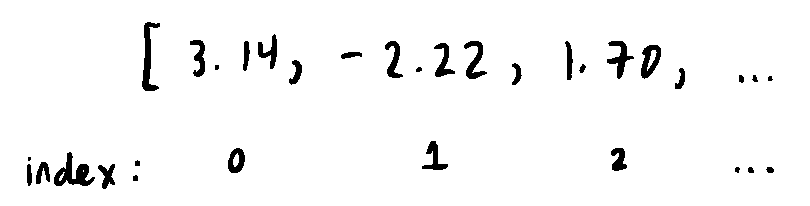
\includegraphics[width=\linewidth]{figs/array.pdf}
  \caption{A generic array, indexed from 0.} 
  \label{fig:array}
\end{figure}

From now on, we will try to think about data storage from the programming
side. From the programming side of things, it is often efficient and intuitive
to organize data such that lots of related information is kept close together.
The most common way to do this is an {\it array}\index{array}, which is
basically an ordered tuple\footnote{In Python, basic arrays are implemented as
lists.}. The $0\nth$ element of an array corresponds to that array's memory
address, and the addresses of all other data stored in that array are measured
relative to the address of this $0\nth$ element. Each element of an array is
labelled with an {\it index}, and one uses index $i$ to access array element
$i$. This is shown schematically in \figref{fig:array}.


The fundamental object we need to store is an $\SU(3)$ gauge field.
From \secref{sec:fields}, recall that this means we must associate four matrices
to each space-time point (because we live in four dimensions). Moreover each
matrix can be represented in a computer as an array; hence the overall
strategy is to create an ``array of subarrays".

Let us begin by storing a matrix in an array. This is relatively
straightforward. An $\SU(3)$ matrix is a $3\times3$ matrix with complex entries,
so a generic matrix $U_\mu(\fvec{x})\in\SU(3)$ at space-time site $\fvec{x}$
pointing in the $\muh$-direction can be represented with 18 real numbers as
\begin{equation}
U_\mu(\fvec{x})=\left(\begin{array}{ccc}
x_{00} + iy_{00} & x_{01} + iy_{01} & x_{02} + iy_{02} \\
x_{10} + iy_{10} & x_{11} + iy_{11} & x_{12} + iy_{12} \\
x_{20} + iy_{20} & x_{21} + iy_{21} & x_{22} + iy_{22} 
\end{array}\right),
\end{equation}
where each $x_{ij},y_{ij}\in\R$. This can be straightforwardly converted to an
18-component array of the form
\begin{equation}
[x_{00},~y_{00},~x_{01},~y_{01},~...,~x_{22},~y_{22}],
\end{equation}
and in practice this is exactly how we store each matrix as an array.

\begin{figure}
  \centering
  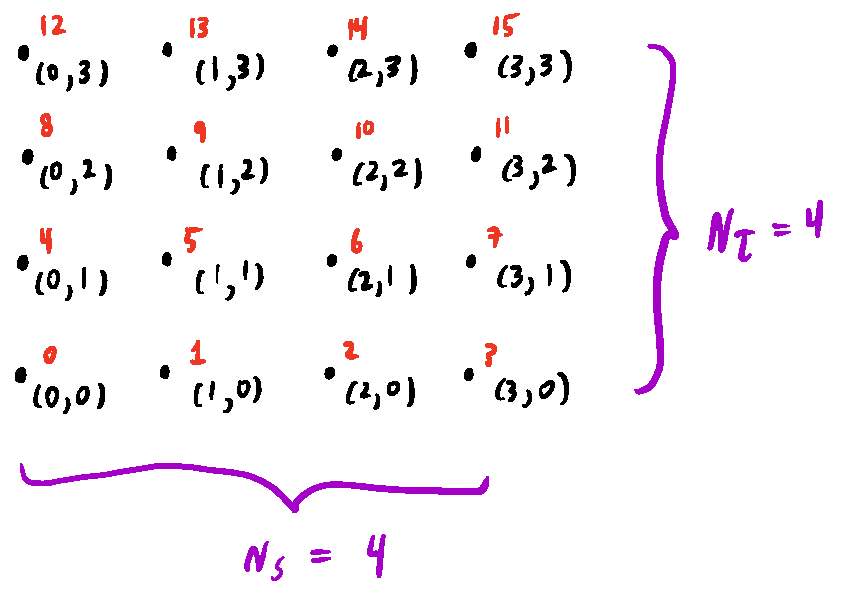
\includegraphics[width=\linewidth]{figs/indexing.pdf}
  \caption{How the sites of a lattice are indexed. In the above example, we
consider a 2-$d$ lattice with spatial extension $N_s=4$ and time extension
$N_\tau=4$. Each site is represented by a black dot and its 2-$d$ coordinate is
listed next to it. The site index is given in red.}
  \label{fig:index}
\end{figure}

Next we will need a way to assign an integer to a space-time coordinate. This is 
called {\it indexing}, and the way indexing goes is shown in \figref{fig:index},
which is a 2-$d$ example. By eye we can see the indexing pattern: we start with
sites at the ``bottom" of the lattice (at $t=0$), then increase our index as we
proceed from left to right (increasing $x$ from 0 to $N_s$). 
In 2-$d$, you can easily verify that the formula that accomplishes this is
\begin{equation}\label{eq:lex2d}
  \text{index}=x+yN_s.
\end{equation}
In four dimensions, this can be generalized to
\begin{equation}\label{eq:lex4d}
  \text{index}=x+yN_s+zN_s^2+tN_s^3.
\end{equation}
This indexing method is called {\it lexicographic
ordering}\index{lexicographic}. 

We are now ready to construct our array of subarrays. Let us call the array
containing the subarrays the ``superarray"\footnote{This is not common
terminology; I'm just trying to be pedagogical. Usually we simply refer to the
``superarray" as the ``gauge field".}. In our case, each subarray contains
the elements of a single link, which again is an $\SU(3)$ matrix.
We will organize our superarray such that all links pointing in the
$\hat{x}$-direction come first, followed by all the $\hat{y}$-links, then the
$\hat{z}$-links, then the $\hat{t}$-links\footnote{In principle there is no 
single ``correct" way to organize the links inside the
superarray; indeed the optimal ordering depends on details of the code. In many
code bases, when accessing links, one loops over the space-time directions. In
that case, having all data corresponding to a particular direction ``close
together" in memory saves a lot of computational effort, because the code has to
spend less time looking up links.}. Schematically, our superarray then looks
like
\begin{equation}
  \text{superarray}=\left[\{U_x\},~\{U_y\},~\{U_z\},~\{U_t\}\right],
\end{equation}
where $\{U_x\}$ indicates the set of all links pointing in the
$\hat{x}$-direction, and similarly for the other sets.
Each set $\{U_x\}$ then stores links $U_x(\fvec{x})$ in this order: according to
\equatref{eq:lex4d}, the link with index 0 comes first, followed by 1, and so
on. Hence this set is ordered like
\begin{equation}
\{U_x\} = \{ U_x(0),~U_x(1),~...,~U_x(N_s^3N_t-1)\},
\end{equation}
where now the argument of each $U$ is its lexicograhic index rather than its
space-time coordinate. This specifies completely how to store an $\SU(3)$ gauge
field in a large array.

To wrap up, let's figure out how large this array must be. Recall that each
$\SU(3)$ matrix in our implementation is represented by 18 real numbers.
If a real number is stored as a double-precision number, that number requires 8
bytes of memory. The total memory requirement for one $\SU(3)$ gauge field is then
\begin{equation}
\text{size}=\text{size of real}\times\text{number of dimensions}
             \times\text{ number of sites.}
\end{equation}
In four dimensions, the number of sites is $N_s^3N_t$, and so 
\begin{equation}\label{eq:latsize}
\text{size}=32N_s^3N_t\text{ bytes.}
\end{equation}

\section{Further studying}

If you have decided you
find lattice calculations interesting, so much so that you think you want to
pursue lattice research in grad school, I would recommend the following books on
the subject:
\begin{itemize}
\item {\it Quantum Chromodynamics on the Lattice: An Introductory Presentation}
by Gattringer and Lang~\cite{gattringer_quantum_2010} is probably the most pedagogical 
introduction to lattice calculations.
\item {\it Quantum Fields on a Lattice} by Montvay and 
M\"unster~\cite{montvay_quantum_1994} is a bit more
rigorous than Gattringer and Lang and contains a few other topics, like the
Higgs phase diagram. It is less pedagogical.
\item {\it Lattice Methods for Quantum Chromodynamics} by DeGrand and 
DeTar~\cite{degrand_lattice_2006} is
an excellent resource for a beginner and contains some extra information about
Symanzik improvement and lattice algorithms.
\end{itemize}
Some other books include Rothe's {\it Lattice Gauge Theories: An 
Introduction}~\cite{rothe_lattice_2005} and Smit's {\it Introduction to Quantum 
Fields on a Lattice}~\cite{smit_introduction_2002}. A book that rather
nicely connects LFT to {\it heavy-ion} experiments\index{heavy-ion experiment},
where we collide heavy nuclei like gold together in order to learn something
about strong interactions experimentally, can be found
in {\it The Deconfinement Transition of QCD: Theory Meets Experiment}
\cite{ratti_deconfinement_2021}. It will probably
be useful to you to at least have digital copies of all of them. In my
experience, when learning an extremely esoteric subject, it helps to have as
many references as possible so that you can see things explained in multiple
different ways.

Lattice calculations lie at the intersection of many disciplines in math,
physics, and scientific computing. Therefore if you want to get a deeper
understanding of the field, you should at least take courses that teach
\begin{itemize}
  \item calculus of more than one variable;
  \item linear algebra;
  \item differential equations;
  \item complex analysis;
  \item probability and statistics;
  \item numerical methods;
  \item special relativity;
  \item thermodynamics;
  \item statistical mechanics;
  \item electrodynamics;
  \item quantum mechanics; and
  \item quantum field theory.
\end{itemize}
If you have time, you can get an even deeper understanding of some niche topics
in the field if you also take courses that cover
\begin{itemize}
  \item topology;
  \item differential geometry;
  \item Lie groups;
  \item clean coding and object-oriented programming;
  \item accelerated computing;
  \item machine learning;
  \item phase transitions and critical phenomena;
  \item general relativity; and
  \item topical courses in contemporary particle physics.
\end{itemize}

I hope that you do choose to become a lattice practitioner. It's a big field
with lots of valuable knowledge, lots of ways to contribute depending on your
skills and interests, and the potential to have some role helping advance modern
particle physics. Thanks for reading these notes. I hope they were helpful to
you in some way.\\[5mm]
-David

\section*{Exercises}
\begin{enumerate}
  \item Looking at \equatref{eq:lex2d} and \eqref{eq:lex4d}, what do you think
should be the lexicographic indexing formula in 3-$d$? Draw a $4\times4\times4$
cube and verify that your formula works.
  \item The Fermilab-MILC-HPQCD collaboration generates some sizeable lattices.
One set of lattices has $N_s=144$ and $N_\tau=288$. Assuming the $\SU(3)$ gauge
field of this configuration is stored in
double precision, how many bytes are required? What about single precision?
\end{enumerate}

\bibliographystyle{unsrtnat}
\bibliography{bibliography}



\printindex


\end{document}
